\begin{filecontents*}{wiley-article.cls}
%%%%%%%%%%%%%%%%%%%%%%%%%%%%%%%%%%%%%%%%%%%%%%%%%%%%%%%
% wiley-article.cls, v1.1, 2017/05/26
% Developed by Overleaf.
%%%%%%%%%%%%%%%%%%%%%%%%%%%%%%%%%%%%%%%%%%%%%%%%%%%%%%%
\NeedsTeXFormat{LaTeX2e}
\ProvidesClass{wiley-article}[2017/05/26, v1.1]
\def\@jlogo{}\def\@jname{}\def\@jyear{}\def\@jpages{}\def\@jvolume{}\def\@jwebsite{}
\def\@runningauthor{}\def\@corraddress{}\def\@corremail{}\def\@presentaddress{}
\def\@papertype{original article}\def\@paperfield{}\def\@paperdoi{}\def\@paperreceived{}\def\@paperrevised{}\def\@paperaccepted{}\def\@papereditor{}
\newif\if@numrefs\newif\if@alpharefs\newif\if@amsrefs\newif\if@blindreview
\DeclareOption{num-refs}{\@numrefstrue\@alpharefsfalse\@amsrefsfalse}
\DeclareOption{alpha-refs}{\@numrefsfalse\@alpharefstrue\@amsrefsfalse}
\DeclareOption{ams-refs}{\@numrefsfalse\@alpharefsfalse\@amsrefstrue}
\DeclareOption{blind}{\@blindreviewtrue}
\ExecuteOptions{num-refs}\ProcessOptions\relax
\LoadClass[twoside]{article}

\RequirePackage[table]{xcolor}\RequirePackage{ifpdf}\RequirePackage{ifxetex}\RequirePackage{ifluatex}
\RequirePackage{mathtools}\RequirePackage{bm}\RequirePackage{graphicx}\RequirePackage{tabularx}
\RequirePackage{textcase}\RequirePackage{dashrule}\RequirePackage{ragged2e}\RequirePackage{authblk}
\RequirePackage[hyphens]{url}\RequirePackage{soul}\RequirePackage{xpatch}
\newif\ifxetexorluatex
\ifxetex\xetexorluatextrue\else\ifluatex\xetexorluatextrue\else\xetexorluatexfalse\fi\fi
\ifxetexorluatex\RequirePackage[framemethod=tikz]{mdframed}\else\ifpdf\RequirePackage[framemethod=tikz]{mdframed}\else\RequirePackage[framemethod=default]{mdframed}\RequirePackage{tikz}\fi\fi
\RequirePackage{silence}\WarningFilter{microtype}{tracking amount list}\WarningFilter{latex}{Reference `mdf@pagelabel}
\ifxetexorluatex
  \RequirePackage{microtype}\RequirePackage{fontspec}\RequirePackage[partial=upright]{unicode-math}
  \setmainfont[Ligatures=TeX]{Arial}\setsansfont[Ligatures=TeX]{Arial}
  %\setmathfont{TeX Gyre DejaVu Math}\setmathfont[range={\int}]{Latin Modern Math}
\else
  \RequirePackage{microtype}\RequirePackage[T1]{fontenc}\RequirePackage[utf8]{inputenc}\RequirePackage[default]{lato}
  \IfFileExists{newtxsf.sty}{\RequirePackage[cmintegrals,nosymbolsc]{newtxsf}}{}
  \ifpdf\SetTracking[spacing={500*,166,}]{encoding={*}}{80}\fi
\fi
\RequirePackage[paperwidth=171mm,paperheight=246mm,left=14.3mm,textwidth=142.4mm,lines=47,headsep=\baselineskip,headheight=16\p@,footskip=23\p@]{geometry}
\RequirePackage{alphalph}\newalphalph{\fnsymbolmult}[mult]{\@fnsymbol}{5}
\newcounter{authorfn}\setcounter{authorfn}{1}\newcommand{\authfn}[1]{\fnsymbolmult{#1}}
\newcommand{\presentadd}[2][]{
  \ifx\empty\@presentaddress\else\appto{\@presentaddress}{\\}{}{}\fi
  \appto{\@presentaddress}{\ifx\empty#1\else\textsuperscript{#1}\fi#2}{}{}
}
\newcommand{\jlogo}[1]{\def\@jlogo{#1}}\newcommand{\jname}[1]{\def\@jname{#1}}\newcommand{\jyear}[1]{\def\@jyear{#1}}\newcommand{\jvolume}[1]{\def\@jvolume{#1}}\newcommand{\jpages}[1]{\def\@jpages{#1}}\newcommand{\jwebsite}[1]{\def\@jwebsite{#1}}
\newcommand{\runningauthor}[1]{\def\@runningauthor{#1}}\newcommand{\corraddress}[1]{\def\@corraddress{#1}}\newcommand{\corremail}[1]{\def\@corremail{#1}}

\newcommand{\paperdoi}[1]{\def\@paperdoi{#1}}\newcommand{\paperreceived}[1]{\def\@paperreceived{#1}}\newcommand{\paperrevised}[1]{\def\@paperrevised{#1}}\newcommand{\paperaccepted}[1]{\def\@paperaccepted{#1}}\newcommand{\papereditor}[1]{\def\@papereditor{#1}}\newcommand{\papertype}[1]{\def\@papertype{#1}}\newcommand{\paperfield}[1]{\def\@paperfield{#1}}
\RequirePackage{scrextend}\changefontsizes[13\p@]{8\p@}
\ifxetexorluatex\newcommand{\allcaps}[2][10.0]{\addfontfeature{LetterSpace=#1}\MakeTextUppercase{#2}}\renewcommand{\textsc}[1]{{\addfontfeature{LetterSpace=10.0,Scale=0.8}\MakeTextUppercase{#1}}}\else\ifpdf\newcommand{\allcaps}[2][]{\textls*[#1]{\MakeTextUppercase{#2}}}\else\newcommand{\allcaps}[2][]{\MakeTextUppercase{#2}}\fi\fi
\RequirePackage[explicit]{titlesec}
\titleformat{\section}{\fontsize{10pt}{13\p@}\bfseries}{\thesection}{1em}{\textmd{|}\quad\allcaps{#1}}
\newcommand{\backmatter}{\titleformat{\section}{\fontsize{10pt}{13\p@}\bfseries}{}{0pt}{\allcaps{##1}}\titlespacing*{\section}{0pt}{ 1.5\baselineskip}{0.5\baselineskip}}
\ifxetexorluatex\titleformat{name=\section,numberless}{\fontsize{10pt}{13\p@}\bfseries}{}{0pt}{\textsc{#1}}\else\ifpdf\titleformat{name=\section,numberless}{\fontsize{10pt}{13\p@}\scshape\bfseries}{}{0pt}{\textls*{#1}}\else\titleformat{name=\section,numberless}{\fontsize{10pt}{13\p@}\scshape\bfseries}{}{0pt}{#1}\fi\fi
\titlespacing*{\section}{0pt}{1.5\baselineskip}{\baselineskip}\titlespacing*{name=\section,numberless}{0pt}{1.5\baselineskip}{0.5\baselineskip}
\titleformat{\subsection}{\fontsize{10pt}{13\p@}\bfseries}{\thesubsection}{1em}{\textmd{|}\quad#1}\titlespacing*{\subsection}{0pt}{1.5\baselineskip}{0.5\baselineskip}
\titleformat{\subsubsection}{\fontsize{10pt}{13\p@}\bfseries}{\thesubsubsection}{1em}{\textmd{|}\quad#1}\titlespacing*{\subsubsection}{0pt}{1.5\baselineskip}{0.5\baselineskip}
\ifxetexorluatex\titleformat{\paragraph}[hang]{\fontsize{8.5\p@}{13\p@}\fontspec{Arial}\color{black!75}}{\theparagraph}{0pt}{#1}\titleformat{name=\paragraph,numberless}[hang]{\fontsize{8.5\p@}{13\p@}\fontspec{Arial}}{}{0pt}{#1}\else\titleformat{\paragraph}[hang]{\fontsize{8.5\p@}{13\p@}\fontseries{eb}\selectfont\color{black!75}}{\theparagraph}{0pt}{#1}\titleformat{name=\paragraph,numberless}[hang]{\fontsize{8.5\p@}{13\p@}\fontseries{eb}\selectfont}{}{0pt}{#1}\fi
\titlespacing*{\paragraph}{0pt}{\baselineskip}{0pt}
\RequirePackage[flushmargin,bottom]{footmisc}\def\blfootnote{\gdef\@thefnmark{}\@footnotetext}\appto{\footnotelayout}{\fontsize{6\p@}{9\p@}\selectfont\itshape}\renewcommand{\footnoterule}{\noindent\textcolor{black!50}{\rule{\textwidth}{0.5\p@}}\vskip2\p@}
\RequirePackage{fancyhdr}\fancyhf{}\renewcommand{\headrule}{}\fancyhead[LO]{{\fontsize{7\p@}{13\p@}\selectfont\setlength{\arrayrulewidth}{.5\p@}\arrayrulecolor{black}\begin{tabularx}{\textwidth}{@{}X r | r @{}}\@runningauthor & & \thepage\\\hline\end{tabularx}}}
\fancyhead[LE]{{\fontsize{7\p@}{13\p@}\selectfont\setlength{\arrayrulewidth}{.5\p@}\arrayrulecolor{black}\begin{tabularx}{\textwidth}{@{}l | l >{\raggedleft\arraybackslash}X @{}}\thepage & & \@runningauthor\\\hline\end{tabularx}}}
\fancypagestyle{firstpage}{\fancyhead[L]{\fontsize{7\p@}{13\p@}\selectfont\setlength{\arrayrulewidth}{.5\p@}\arrayrulecolor{black}\begin{tabularx}{\textwidth}{@{}l | l | X @{}}\ifdefempty{\@paperreceived}{\multicolumn{3}{l}{}}{Received: \@paperreceived & Revised: \@paperrevised & Accepted: \@paperaccepted}\\\hline\ifdefempty{\@paperdoi}{}{\multicolumn{3}{@{}l}{DOI: \@paperdoi}}\end{tabularx}}\fancyfoot[L]{\fontsize{7\p@}{13\p@}\selectfont\begin{tabularx}{\textwidth}{@{}X  >{\centering\arraybackslash}X  r | r @{}}\hline\ifdefempty{\@paperreceived}{& & & }{\textit{\@jname}~\@jyear; \@jvolume: \@jpages & \@jwebsite & \textcopyright~\@jyear\space Wiley Periodicals, Inc. & }\thepage\end{tabularx}}}
\newcommand{\contrib}[2][]{\blfootnote{\textsuperscript{#1}#2}}
\setcounter{Maxaffil}{1}\renewcommand{\Authsep}{\quad|\quad}\renewcommand{\Authand}{\quad|\quad}\renewcommand{\Authands}{\quad|\quad}\renewcommand{\Authfont}{\fontsize{12\p@}{20pt}\bfseries\raggedright}\renewcommand{\Affilfont}{\fontsize{7\p@}{10pt}\selectfont\raggedright}\renewcommand\AB@authnote[1]{\textsuperscript{#1}}\patchcmd{\AB@affilsepx}{\\}{\\[3\p@]}{}{}\patchcmd{\@author}{\AB@authlist\\[\affilsep]\AB@affillist}{\AB@authlist}{}{}
\renewcommand{\maketitle}{
  \if@blindreview\def\AB@authlist{\Authfont Anonymous Authors}\def\AB@affillist{\Affilfont Anonymous Affiliations}\def\@runningauthor{Authors (Anon)}\def\@corraddress{Anon correspondence}\def\@corremail{anon@example.com}\def\@presentaddress{Anon present address}\fi
  \vspace*{\dimexpr 27\p@-2\baselineskip}\noindent\begingroup\setul{3\p@}{1\p@}\ifxetexorluatex\fontspec{Arial}\else\fontseries{eb}\selectfont\fi{\fontsize{9\p@}{15\p@}\allcaps[\ifxetexorluatex 20\else 200\fi]{\ul{\@papertype}}}\ifdefempty{\@jlogo}{\rule{0pt}{2em}}{\hfill\includegraphics[height=2em]{\@jlogo}}\\[2\p@]{\fontsize{8\p@}{15\p@}\ifxetexorluatex\addfontfeature{LetterSpace=20.0}\@paperfield\else\ifpdf\textls*[150]{\@paperfield}\else\@paperfield\fi\fi}\endgroup\vskip13\p@{\fontsize{18\p@}{23\p@}\bfseries\raggedright\@title\par}\vskip27\p@\noindent\begin{minipage}{0.8\textwidth}\@author\end{minipage}\vskip21\p@\thispagestyle{firstpage}
}
\newcommand{\wiley@affilmetadata}{\AB@affillist\par\vskip10pt\textbf{Correspondence}\\\@corraddress\\Email: \@corremail\par\ifx\empty\@presentaddress\else\vskip10pt\textbf{Present address}\\\@presentaddress\par\fi\vskip10pt\par\ifdefempty{\@papereditor}{}{\vskip10pt Editor: \@papereditor\par}}
\newcommand{\abbrevs}[1]{\blfootnote{\textbf{Abbreviations:} #1\\[-3\p@]}}
\RequirePackage{changepage}\RequirePackage{environ}\reversemarginpar\newlength{\wiley@affilmetadataheight}\newlength{\wiley@abstractheight}
\NewEnviron{wiley@abstract}{
  \newcommand{\keywords}[1]{\vskip8\p@\noindent{\bfseries\fontsize{7\p@}{13\p@}\allcaps[\ifxetexorluatex 20\else 200\fi]{keywords}\par}\noindent{\raggedright\fontsize{8\p@}{13\p@}\selectfont ##1\par}}
  \strictpagecheck\begin{adjustwidth*}{\dimexpr 54.9mm-6.5\p@}{}\setlength{\marginparsep}{-47mm}\setlength{\marginparwidth}{47mm}\settototalheight{\wiley@affilmetadataheight}{\parbox{\marginparwidth}{\wiley@affilmetadata}}\newsavebox{\wiley@abstractbox}\savebox{\wiley@abstractbox}{\parbox{\linewidth}{\begin{mdframed}[font=\fontsize{9\p@}{15\p@}\selectfont,topline=false,bottomline=false,leftline=true,rightline=false,backgroundcolor=black!10,middlelinewidth=6\p@,middlelinecolor=white,outerlinewidth=0.5\p@]\BODY\end{mdframed}}}
  \settototalheight{\wiley@abstractheight}{\usebox{\wiley@abstractbox}}\marginpar{\wiley@affilmetadata}\vskip-1.5em\begin{mdframed}[font=\fontsize{9\p@}{15\p@}\selectfont,topline=false,bottomline=false,leftline=true,rightline=false,backgroundcolor=black!10,middlelinewidth=6\p@,middlelinecolor=white,outerlinewidth=0.5\p@]\BODY\end{mdframed}\ifdimgreater{\wiley@affilmetadataheight}{\wiley@abstractheight}{\vskip\dimexpr\wiley@affilmetadataheight-\wiley@abstractheight+\baselineskip\relax}{}
}[\end{adjustwidth*}]\renewcommand{\abstract}{\wiley@abstract}\renewcommand{\endabstract}{\endwiley@abstract}
\RequirePackage{quoting}\quotingsetup{vskip=\baselineskip,indentfirst=false,font={itshape,RaggedRight,normalsize},leftmargin=26\p@,rightmargin=26\p@}\renewenvironment{quote}{\begin{quoting}}{\end{quoting}}\renewenvironment{quotation}{\begin{quoting}}{\end{quoting}}
\RequirePackage[inline]{enumitem}\setlist{nosep,font=\bfseries,leftmargin=*,align=left}\setlist[1]{topsep=\baselineskip,leftmargin=\parindent,labelsep=*,labelwidth=*}
\RequirePackage[tableposition=top]{caption}\DeclareCaptionFont{captionfont}{\fontsize{8\p@}{11\p@}\selectfont}\DeclareCaptionFont{boxcaption}{\fontsize{9\p@}{13\p@}\selectfont}
\ifxetexorluatex\DeclareCaptionFont{heavy}{\fontspec{Arial}}\DeclareCaptionLabelFormat{allcaps}{\addfontfeature{LetterSpace=15.0}{\MakeTextUppercase{#1}~#2}}\else\DeclareCaptionFont{heavy}{\fontseries{eb}}\ifpdf\DeclareCaptionLabelFormat{allcaps}{\textls[150]{\MakeTextUppercase{#1}~#2}}\else\DeclareCaptionLabelFormat{allcaps}{\MakeTextUppercase{#1}~#2}\fi\fi
\captionsetup*{justification=raggedright,singlelinecheck=false,font=captionfont,labelformat=simple,labelfont=bf,labelsep=space}\captionsetup*[table]{skip=0.5ex}
\AtBeginEnvironment{table}{\fontsize{7.5\p@}{10.5\p@}\selectfont\rowcolors*{3}{black!10}{}\renewcommand{\arraystretch}{1.25}\arrayrulecolor{black!20}\setlength{\arrayrulewidth}{1\p@}}
\RequirePackage{threeparttable}\renewcommand{\TPTnoteSettings}{\leftmargin=0pt}\newcommand{\headrow}{\rowcolor{black!20}}\newcommand{\thead}[1]{\multicolumn{1}{l}{\bfseries #1\rule[-1.2ex]{0pt}{2em}}}
\if@numrefs\RequirePackage[numbers]{natbib}\fi
\if@alpharefs\RequirePackage{natbib}\fi
\if@amsrefs\RequirePackage{amsrefs}\let\citep\cite\let\citet\ocite\renewcommand{\biblistfont}{\fontsize{7.5\p@}{10.5\p@}\selectfont}\fi
\AtBeginDocument{\@ifpackageloaded{natbib}{\setlength{\bibhang}{1.5em}\renewcommand{\bibfont}{\fontsize{7.5\p@}{10.5\p@}\selectfont}\renewcommand{\refname}{References}\renewcommand{\bibname}{References}}{}}
\RequirePackage{lettrine}\newenvironment{biography}[2][]{\begin{mdframed}[linewidth=0.5\p@,skipabove=1.5\baselineskip,innerleftmargin=6\p@,innerrightmargin=6\p@,innertopmargin=6\p@,innerbottommargin=6\p@]\ifstrequal{#1}{}{}{\lettrine[image,lines=5,findent=1em,nindent=0pt]{#1}{}}\bfseries\scshape #2}{\end{mdframed}}
\normalsize\pagestyle{fancy}
\end{filecontents*}

\documentclass[num-refs]{wiley-article}
\usepackage{amsmath,graphicx,booktabs,hyperref,siunitx,xspace,tabularx,multirow,array,float,placeins,caption,threeparttable}
\usepackage[nameinlink]{cleveref}
\usepackage{xcolor}
\captionsetup{font=small,labelfont=bf,labelformat=simple,labelsep=space}
\newcommand{\rev}[1]{\textcolor{blue}{#1}}

% Footnotes in italics
\makeatletter
\renewcommand{\footnotelayout}{\fontsize{6\p@}{9\p@}\selectfont\itshape}
\makeatother

% Bold cross-reference labels for Tables and Figures
\crefformat{table}{\textbf{Table~#2#1#3}}
\Crefformat{table}{\textbf{Table~#2#1#3}}
\crefformat{figure}{\textbf{Figure~#2#1#3}}
\Crefformat{figure}{\textbf{Figure~#2#1#3}}
\crefname{table}{\textbf{Table}}{\textbf{Tables}}
\Crefname{table}{\textbf{Table}}{\textbf{Tables}}
\crefname{figure}{\textbf{Figure}}{\textbf{Figures}}
\Crefname{figure}{\textbf{Figure}}{\textbf{Figures}}
\crefname{equation}{Equation}{Equations}
\Crefname{equation}{Equation}{Equations}
\crefname{section}{Section}{Sections}
\Crefname{section}{Section}{Sections}
\crefname{subsection}{Section}{Sections}
\Crefname{subsection}{Section}{Sections}
% Bold autoref names for tables and figures
\renewcommand{\figureautorefname}{\textbf{Figure}}
\renewcommand{\tableautorefname}{\textbf{Table}}

\title{Legalyze: An Open-Source Structure-Aware Agentic RAG Platform for High-Precision Legal Intelligence}
\author[1*]{Ali Hamza}
\author[1]{Maaz Bin Rizwan}
\author[1]{Maemoona Kayani}
\author[1]{Shafa-at Ali Sheikh}
\affil[1]{Department of Software Engineering, National University of Sciences and Technology (NUST), Islamabad, Pakistan}
\corraddress{*Ali Hamza, NUST, Islamabad, Pakistan}
\corremail{ahamza.msse25mcs@student.nust.edu.pk}
\runningauthor{Hamza et al., (2026)}

\begin{document}
\raggedbottom

\maketitle
\begin{abstract}
The integration of Large Language Models into the legal domain is constrained by a
reliability gap, where models can generate incorrect or unsupported information in
specialized reasoning tasks. This issue is especially important in jurisdictions such
as Pakistan, where legal texts have strong structural dependencies and require accurate
grounding. This research introduces Legalyze, an open-source and modular five-tier
system designed to support legal analysis. The system uses Structure-Aware Hierarchical
Indexing (SAHI) and a dual-stream retrieval pipeline that combines lexical and semantic
search using Reciprocal Rank Fusion. It also includes a component called Legal Wisdom of
Extraction, which identifies key legal entities such as petitioners, respondents, court
names, and referenced laws from the text. By preserving the structure of legal documents
and grounding responses in retrieved evidence, the system substantially improves the
grounding of generated outputs. Evaluation on a 1.2 million-token corpus of Pakistani
statutes and case law, comprising five statutory and case-law sources with 67 legal
queries assessed by three independent legal reviewers under a reviewer-blinded evaluation
protocol (Fleiss' $\kappa = 0.743$, substantial agreement), showing a reduction in
pooled hallucination rates from 54.7\% in a zero-shot baseline to 5.5\%,
outperforming standard retrieval-based approaches. \rev{The improvement over both baselines
is statistically significant across all pairwise comparisons (Cochran's
$Q = 37.57$, $p = 6.93 \times 10^{-9}$; McNemar exact: Zero-Shot vs.\ Legalyze
$p = 5.40 \times 10^{-9}$). A seven-configuration offline retrieval ablation further
demonstrates that an offline surrogate of the Legalyze architecture achieves Recall@5
of 65.0\%, compared to 45.0\% for flat lexical retrieval, confirming the retrieval
gains attributable to structure-aware indexing}. These results show that structure-aware
retrieval combined with targeted information extraction can improve the reliability of
AI systems for legal research and analysis. Legalyze represents a promising prototype
for delivering trustworthy, jurisdiction-specific legal intelligence as a research and
decision-support tool in professional environments.

\keywords{Expert Systems, Natural Language Processing (NLP), Retrieval-Augmented
Generation (RAG), Agentic Systems, Hybrid Retrieval, Knowledge Grounding, Reciprocal
Rank Fusion (RRF), Vector Databases, Multi-Tier Architecture, Hallucination Reduction,
Legal AI, Pakistani Legal Systems}
\end{abstract}


\section{Introduction}
\label{sec:intro}

Law practice is fundamentally an exercise in structured reasoning over authoritative
texts \cite{r9}. Legal professionals, including lawyers, judges, and researchers, interpret statutes, constitutional provisions, judicial precedents, and
procedural rules to provide legal advice and resolve disputes. This process requires
precise interpretation and careful cross-referencing of legal sources. As legal corpora
continue to expand in both volume and complexity, manual legal research has become
increasingly difficult. Professionals must navigate large collections of statutes and
case law while maintaining strict accuracy in citation and interpretation. Although
modern artificial intelligence models can summarize documents and explain legal concepts,
they often generate fabricated laws or incorrect citations, a phenomenon commonly
referred to as ``hallucination.''

Research shows that leading models can produce legal hallucinations at a rate as high as
58\% \cite{r88}. To combat this, Retrieval-Augmented Generation (RAG) is used to ground
AI responses in real documents; however, standard RAG often fails to understand the
hierarchical structure of legal texts. These failures are quantified by experiments
conducted by \cite{r96}, which show that while advanced retrieval can improve
performance, a single-round RAG system may only achieve a recall rate of 74.67\%,
compared to a baseline recall of 57.33\% and a multi-round recall of 78.67\%.
Furthermore, while many nations have developed specialized legal AI, Pakistan currently
lacks a dedicated platform for its national statutes and case law \cite{r43}. Legal AI
initiatives in neighbouring South Asian jurisdictions, including India, Bangladesh, and Nepal, have similarly highlighted the need for jurisdiction-specific, corpus-grounded
platforms tailored to regional legal frameworks \cite{r58}; however, no such
end-to-end open-source platform currently exists for the Pakistani legal system. The
present work addresses this gap exclusively for Pakistani law, and the incorporation
of additional South Asian jurisdictions is identified as a priority for future versions
of the platform.

This research proposes \textbf{Legalyze}, an open-source%
\footnote{\url{https://github.com/ali-Hamza817/Legalyze}} AI-powered platform tailored
specifically for the Pakistani legal ecosystem. Its core technical novelty is
Structure-Aware Hierarchical Indexing (SAHI), a deterministic parsing and indexing
mechanism that annotates each text chunk with a hierarchical breadcrumb (e.g.,
\emph{Part~II, Chapter~1, Article~10A}) before retrieval, thereby substantially improving
hierarchy-aware retrieval and structure preservation throughout the entire intelligence
pipeline. \rev{Combined with a dual-stream retrieval pipeline and a multi-agent reasoning architecture, Legalyze is designed to ground generated claims in verifiable statutory evidence. The evaluation methodology follows a reviewer-blinded protocol over 67 legal queries evaluated across three system configurations, with hallucination traceability independently assessed by three legal reviewers; statistical significance across all paired comparisons is established using omnibus Cochran's $Q$ tests, pairwise exact McNemar tests, and Generalized Estimating Equations (GEE) modeling to account for query clustering.} The primary novelty
of Legalyze is providing the first end-to-end, jurisdiction-specific legal intelligence
solution for Pakistan's unique legal framework. The remainder of this paper is organized
as follows: \Cref{sec:lit} reviews the literature, and \Cref{sec:method} details the
Legalyze methodology, focusing on system architecture, product interfaces, and analysis.
\Cref{sec:results} presents the experimental results, \Cref{sec:discussion} discusses
these findings, and \Cref{sec:conclusion} concludes the paper.


\section{Literature Review}
\label{sec:lit}

The development of legal artificial intelligence has transitioned from early attempts at
modeling reasoning through rules to modern, agent-based architectures that prioritize
verifiable retrieval and jurisdictional precision. A synthesized analysis of the existing
literature within the legal AI domain is presented in \cref{tab:litreview}, which
categorizes previous research based on methodology, key contributions, and identified
technical limitations.

The evolution of the field began with symbolic systems designed to model legal reasoning
through hand-coded logic. In 1991, \cite{r9} established the conceptual foundation of
the field by defining legal practice as an exercise in structured, adversarial reasoning
over authoritative texts and past cases. While his work introduced hypothetical-based
reasoning to simulate legal arguments, the system was limited by its inability to scale
across the massive digital datasets used by modern practitioners \cite{r9}. By 2020,
research shifted toward data-driven methodologies as \cite{r226} provided a
comprehensive taxonomy of legal tasks, such as judgment prediction and information
extraction. This work marked the definitive move from rule-based systems to neural
models, yet these early neural approaches were limited because they could not capture
the deep hierarchical relationships found in law books \cite{r226}.

To bridge the gap between general language and legal terminology, \cite{r171} developed
specialized models like Bidirectional Encoder Representations from Transformers for
Legal in 2020, demonstrating that training AI on legal documents significantly improves
its understanding. Despite this progress, the model was limited because its knowledge
was static; it could not ground its answers in real-time external evidence or new
statutes \cite{r171}. By 2022, a decadal review by \cite{r223} identified that while
technical capabilities had grown, the lack of explainability remained a primary barrier
to judicial adoption. Following this, \cite{r130} introduced the ``Eval-RAG'' framework
in 2023 to verify generated text against retrieved documents. This successfully
identified factual errors missed by standard metrics, but the approach was limited
because its success was entirely dependent on the quality of the initial search step,
which often failed in dense legal databases \cite{r130}.

The year 2024 saw a surge in research aimed at measuring AI unreliability and addressing
regional gaps. \cite{r88} documented that state-of-the-art models hallucinate legal
facts at a rate of 58\%, highlighting the risks for professional use. \cite{r40} further
audited leading research tools and found that they frequently produced ``hallucinated
citations'' that looked real but did not exist. To standardize how we measure these
failures, \cite{r188} introduced ``LegalBench-RAG,'' which revealed that standard AI
search systems often miss critical legal dependencies. Addressing the lack of regional
data identified by these benchmarks, \cite{r43} developed the first bilingual
constitutional dataset for Pakistan, though it was limited to constitutional law.
Concurrently, \cite{r58} explored AI in South Asia, noting that generic architectures
lacked the precision for local litigation. To refine these checks, \cite{r162} found
that 80\% of machine-generated legal analysis contained factual gaps, while \cite{r27}
observed that models struggled to maintain consistent grounding over multi-paragraph
responses. Finally, \cite{r104} demonstrated that Knowledge Graphs could improve legal
recommendations, yet this was limited to specific charge prediction tasks.

The need for jurisdiction-specific legal AI has been further underscored by regional
initiatives across South Asia. In India, projects such as the Indian Legal Service
Intelligence (ILSI) and AI Sanyog have demonstrated the feasibility of NLP-assisted
legal research within civil law frameworks; similar legal chatbot and access-to-justice
initiatives have emerged in Bangladesh \cite{r58} and Nepal. These efforts collectively
confirm that general-purpose language models, without corpus-specific grounding and
structural hierarchy preservation, are insufficient for the precision demands of regional
legal practice. Legalyze~v1.0 addresses this gap specifically for the Pakistani
jurisdiction; extending the platform to cover additional South Asian legal systems is a
planned roadmap item for future versions, as each jurisdiction requires its own statutory
corpus, heading-detection rules, and precedent adjudication hierarchy.

By 2025, research moved toward refining architectures to solve core retrieval and
auditing failures. \cite{r132} emphasized the need for ``professional-grade'' AI with
integrated verification layers. \cite{r96} proposed a multi-round RAG framework that
improved retrieval recall to 78.67\% from a 57.33\% baseline, though it introduced high
computational latency. \cite{r45} identified a ``Document-Level Retrieval Mismatch'' and
proposed summary-augmented methods to provide retrievers with global context.

\textbf{Legalyze} addresses these cumulative limitations by introducing a
structure-aware architecture designed specifically for the Pakistani legal framework. \rev{By
utilizing hierarchical indexing and dual-stream discovery, Legalyze \textit{substantially
improves} the grounding of retrieved claims, mitigating the retrieval mismatches identified
by \cite{r45}. The platform coordinates specialized agents to perform automated auditing
and timeline synthesis, solving the long-form consistency issues noted by \cite{r27}.
By combining high-precision retrieval with agentic auditing, Legalyze reduces the 58\%
hallucination rate documented by \cite{r88} to 5.5\% (pooled across all reviewer
judgments) or 4.5\% (consensus-adjudicated majority vote), a statistically significant
improvement confirmed by Cochran's $Q = 37.57$ ($p = 6.93 \times 10^{-9}$).} This makes
Legalyze the first end-to-end, jurisdiction-specific legal intelligence solution for
Pakistan's unique legal framework.



\renewcommand{\arraystretch}{1.45}

\begin{table*}[t]
\caption{Overview of legal AI research highlighting methodologies, key findings, and unresolved limitations across prior studies.}
\label{tab:litreview}
\centering
\footnotesize
\begin{tabularx}{\textwidth}{|>{\raggedright\arraybackslash}p{2.5cm}|>{\raggedright\arraybackslash}p{3.0cm}|>{\raggedright\arraybackslash}X|>{\raggedright\arraybackslash}X|}
\hline
\rowcolor{black!15}
\textbf{Study} & \textbf{Methodology} & \textbf{Key Findings} & \textbf{Limitations} \\
\hline

Ashley (1991) & Case-Based Reasoning & Defined legal reasoning as structured interpretation over authoritative legal texts and prior cases. & Limited scalability for large digital legal corpora. \\
\hline

Zhong et al. (2020) & Task Taxonomy & Established a taxonomy for legal AI tasks and accelerated the transition toward neural legal systems. & Did not address hallucination or grounding limitations. \\
\hline

Chalkidis et al. (2020) & Domain Pretraining & LEGAL-BERT improved legal language understanding through domain-specific pretraining. & Relied on static knowledge without external retrieval grounding. \\
\hline

Villata et al. (2022) & Review Study & Identified explainability as a major barrier to legal AI adoption. & Did not propose a technical mitigation framework. \\
\hline

Ryu et al. (2023) & Eval-RAG Framework & Retrieval-based verification improved factual consistency in generated responses. & Performance remained dependent on retriever quality. \\
\hline

Dahl et al. (2024) & Empirical Evaluation & Reported hallucination rates approaching 58\% in legal AI systems. & Did not propose an architectural solution. \\
\hline

Magesh et al. (2024) & Audit Study & Demonstrated that commercial legal AI tools frequently generated fabricated citations. & Focused primarily on auditing rather than system development. \\
\hline

Pipitone and Alami (2024) & Benchmarking & Highlighted retrieval gaps and dependency failures in RAG systems. & Did not introduce a retrieval architecture. \\
\hline

Faisal and Yousaf (2024) & Dataset Development & Created the first bilingual Urdu-English constitutional dataset for Pakistan. & Limited exclusively to constitutional law. \\
\hline

Wasi et al. (2024) & Regional Legal AI Study & Identified insufficient precision of generalized AI systems in South Asian litigation contexts. & Generic architectures lacked jurisdiction-specific adaptation. \\
\hline

Hou et al. (2024) & Evaluation Study & Found factual gaps in nearly 80\% of generated legal analyses. & Detection mechanisms remained limited. \\
\hline

Louis et al. (2024) & Long-form Legal QA & Identified grounding inconsistency across multi-paragraph legal responses. & Weak long-form coherence and evidence preservation. \\
\hline

Abuzir (2025) & System Design Analysis & Advocated for verification-integrated professional legal AI systems. & Lacked empirical implementation and validation. \\
\hline

Zhang et al. (2025) & Multi-round RAG & Improved retrieval recall performance through iterative retrieval mechanisms. & Introduced high computational latency. \\
\hline

Reuter et al. (2025) & Retrieval Optimization & Reduced document-level retrieval mismatch using summary-augmented retrieval. & Relied heavily on generated summaries for context preservation. \\
\hline

\end{tabularx}
\end{table*}

\section{Methodology}
\label{sec:method}

\indent Legal intelligence requires the strong preservation of statutory hierarchy in all stages of the processing pipeline, so we built Legalyze strictly following this principle. This research combines domain-specific hierarchical indexing with a multi-tiered agentic retrieval pipeline to convert raw legal statutes into valid, verifiable, and citation-grounded intelligence. This section will clearly explain our product, Legalyze, by categorizing it into 3 subsections: \Cref{subsec:five_tier_infra} (System Architecture) describes the five-tier infrastructure of Legalyze along with the SAHI pipeline, \Cref{subsec:product_interface} (Product Interface) explains the product specification and user interface of Legalyze, and at last \Cref{subsec:analysis} (Analysis) provides a detailed analysis on product performance by setting up evaluation metrics. A video demonstration of the Legalyze platform is also available online\footnote{\normalsize \url{https://www.youtube.com/watch?v=ofoQ3na1cRE}}.

\subsection{System Architecture}
\label{subsec:five_tier_infra}

Legalyze is built using a Service-Oriented Architecture based on five loosely coupled tiers, which eventually result in a modular and scalable product. The architecture of Legalyze is divided into multiple tiers, allowing for the isolation of specific functions. If one service goes down, the others should not be affected. Separation of core system features and supporting features, thereby achieving the SOLID Principles.

\subsubsection{The Five-Tier Infrastructure}

The overall system architecture is shown in \autoref{fig:architecture}, showing the interaction between the user interface and all the other layers of Legalyze. On the basis of modular service separation, the system is subdivided into five logical layers, which address different aspects of the legal intelligence lifecycle. Changes made to the base AI models do not interfere with the client-facing services. Prior to discussing the dynamic data flow, we first examine the structure and layout of the platform's core infrastructure.

\paragraph{\textbf{Tier 1: User Interface}}

React and Vite are used on the front end, and Material UI is used to style the interface. Four main functional surfaces allow practitioners to interact with the system. The Chat Interface accepts natural-language legal questions. The Document Generation module helps in creating legal documents. The Compliance CheckUp screen verifies records against the constitution. The Case Buildup Wizard assists practitioners step by step in creating a well-organized and complete case file.

% -------- Figure 1: System Architecture --------
\begin{figure*}[t!]
    \centering
    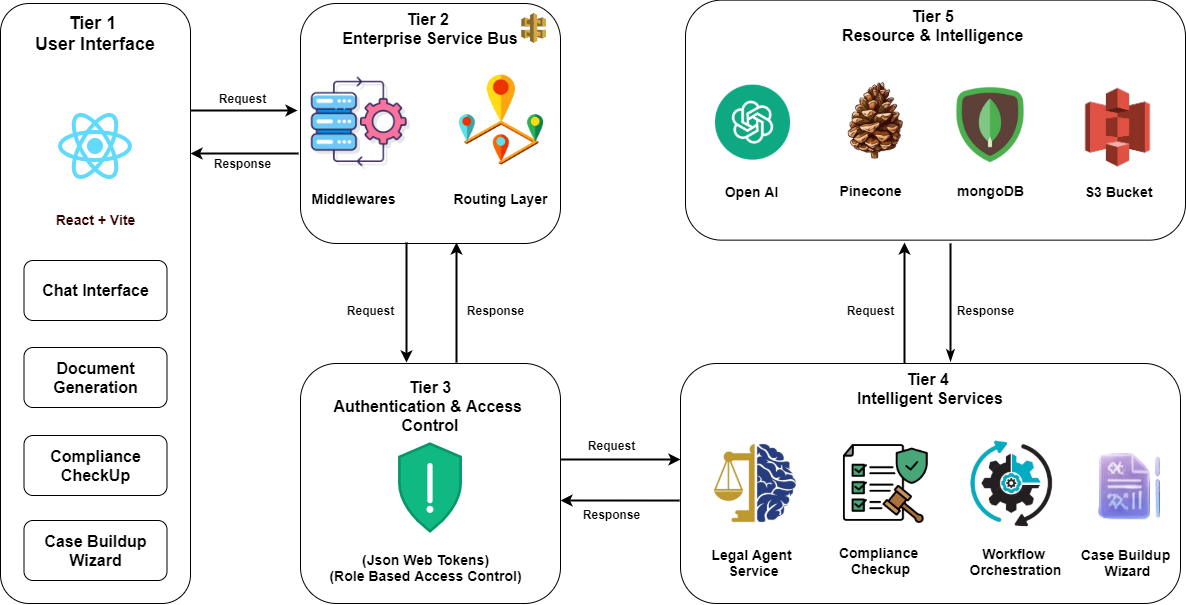
\includegraphics[width=\textwidth]{Architecture Diagram.png}
    \caption{Legalyze follows a five-tier architecture for secure and scalable legal intelligence, where requests originate from the User Interface (Tier 1), pass through the Enterprise Service Bus (Tier 2), are authenticated via JWT-based RBAC (Tier 3), processed by Intelligent Services (Tier 4) for reasoning, compliance, and workflows, interact with the Resource Layer (Tier 5) for LLM processing, retrieval, and storage, and return through the same pipeline to ensure traceable and validated outputs.}
    \label{fig:architecture}
\end{figure*}


\paragraph{\textbf{Tier 2: Enterprise Service Bus}}

The Enterprise Service Bus is an application constructed using Node.js and Express, and it serves as the communication controller of the system. Every query passes through this layer whenever a user presses a button or submits a question. It is developed using modern tools such as Node.js and Express to ensure fast and smooth operation. This layer performs several important functions to keep the system running smoothly. First, it verifies each request to ensure that it is valid and secure before allowing it to proceed. Second, it maintains a detailed log of system activities so that any issues can be identified and resolved. Third, it regulates the rate at which users can submit requests to prevent system overload or crashes. Fourth, it routes data to the appropriate AI service to generate a response.

\paragraph{\textbf{Tier 3: Authentication and Access Control}}

Any request directed to the AI services must first pass through the authentication tier. The system uses JSON Web Tokens to maintain sessions and Google OAuth 2.0 to authenticate practitioners. This layer acts as a security checkpoint, ensuring that only authorized users can access the AI tools. It integrates Google Login to allow users to sign in securely using existing accounts, eliminating the need to store personal passwords and thereby enhancing security. Once authenticated, the system issues a digital token that allows users to access different parts of the system without repeatedly entering credentials. It also uses a rule-based access control mechanism to determine what each user can view and perform. This ensures the confidentiality of sensitive documents and restricts access to critical tools to authorized individuals only. Additionally, it secures the Constitutional Compliance tool, ensuring that only authorized users can perform in-depth audits of legal content. This role-based separation also ensures that all system operations are properly monitored and controlled.

\paragraph{\textbf{Tier 4: Intelligent Services}}

This is the brain of Legalyze, where all the processing takes place. It plans the flow of legal work and manages a team of specialized AI assistants to understand your documents. This layer follows a four-step process when you upload a legal document to handle all the information. First, it extracts text from your file using specialized optical character recognition tools that can read scanned or blurry document images. This helps ensure that text within your documents is captured. Second, the names of important individuals and the relevant laws mentioned in the text are identified using a tool called Legal Wisdom of Extraction (LWOE). It recognizes key entities such as petitioners, respondents, and court names. Third, the Structure-Aware Hierarchical Indexing (SAHI) tool splits large documents into smaller, meaningful fragments so that the AI can process the information more easily without confusion. Each fragment is assigned a unique identifier, or ``breadcrumb,'' so it can always be traced back to its original article or section in the law document. This breadcrumb helps preserve the original structure of the document. The formal parsing algorithm for this step is detailed in Algorithm~1 in \Cref{subsec:sahi_pipeline}. Fourth, these fragments are encoded into numerical representations known as embeddings, allowing them to be retrieved instantly when a query is made. These embeddings enable fast and accurate searches. This layer also includes specialized AI agents that can automatically classify the type of document, such as a police report (FIR) or a court judgment. These agents categorize documents quickly and accurately. It can also construct a timeline to show how events occurred in a case, helping users understand the overall sequence of legal actions. This chronological view provides a clearer understanding of the case. Finally, it offers an audit tool that checks whether legal writing complies with the rules of the Pakistani Constitution. If any part is incorrect, the system highlights it and shows the relevant law so corrections can be made before submission. This helps reduce legal errors. All these services work together to make legal research faster and more reliable.

\paragraph{\textbf{Tier 5: Resource and Intelligence}}
This layer provides the computing infrastructure of the system. GPT-4o is used as the main reasoning model for complex generation tasks. GPT-4o-mini is used for lower-complexity extraction tasks at reduced cost. Pinecone Serverless is used to store vector embeddings, which can be filtered by metadata and accessed by statute, jurisdiction, or court level \cite{r600}. MongoDB Atlas stores structured metadata, user data, case summaries, and immutable audit logs. AWS S3 is used to store original legal PDF documents, and pre-signed URLs with time limits ensure that document access remains authenticated and auditable at each step. Collectively, these resources form the core infrastructure of Legalyze, enabling all dependent services, processing layers, and user-facing features to operate smoothly and reliably across the platform \cite{r605}.

\subsubsection{SAHI, Dual-Stream Discovery, and the RRF Pipeline}
\label{subsec:sahi_pipeline}

A three-stage retrieval pipeline is the most technically unique aspect of Legalyze.
\autoref{fig:dataflow} shows the entire process, starting with the ingestion of raw
statutes and ending with the generation of grounded answers. This pipeline is
independent of the static tiering in order to achieve high-precision knowledge
grounding.

A raw legal PDF is initially processed by the SAHI module, as indicated in
\autoref{fig:dataflow}. SAHI produces two annotations for each chunk of text. The
semantic anchor of the chunk identifies the main legal concept covered by that chunk.
A hierarchical breadcrumb records the structural location of the chunk within the
source document, e.g., Constitution of Pakistan, Part~II, Chapter~1, Article~10A.
Both annotations are stored in MongoDB, where they can be retrieved by key, and in
Pinecone along with the vector embedding, where they can be retrieved semantically.

To formalize this indexing process, the complete SAHI parsing protocol is specified in
Algorithm~1. The parser operates deterministically on raw statutory text using
regular-expression rules targeting Pakistani legal formatting conventions (e.g.,
\texttt{\^{}PART [IVX]+}, \texttt{\^{}CHAPTER [0-9]+},
\texttt{\^{}\textbackslash s*([0-9]+[A-Z]*).\textbackslash s+([A-Z].*)}). Semantic
anchors are derived directly from the nearest detected heading text without requiring an external LLM
is involved in this step. Each chunk is stored with the metadata record
\texttt{\{chunk\_id, breadcrumb, semantic\_anchor, source\_doc, page\_number,
token\_count\}}.

\begin{figure}[H]
\centering
\begin{minipage}{0.95\linewidth}
\hrule
\vspace{0.5em}
\textbf{Algorithm 1: Structure-Aware Hierarchical Indexing (SAHI) Parser}
\vspace{0.5em}
\hrule
\vspace{0.5em}
\begin{verbatim}
Input: raw_text (Full statutory/constitutional document)
Output: chunks (List of structurally annotated, embedded chunks)

1: Initialize state variables:
   current_part = "", current_part_name = ""
   current_chapter = "", current_article = null
   current_text = [], chunk_idx = 0, chunks = []
2: Locate content_start_line (skip Table of Contents by
   finding first "PART I")
3: For each line in raw_text from content_start_line to end:
4:    If line matches PART_PATTERN (e.g., "^PART [IVX]+"):
5:       SaveCurrentArticle(current_article, current_text)
6:       current_part = regex_group(1)
7:       current_part_name = regex_group(2) or read_next_line()
8:       Continue
9:    If line matches CHAPTER_PATTERN (e.g., "^CHAPTER [0-9]+"):
10:      SaveCurrentArticle(current_article, current_text)
11:      current_chapter = regex_group(1)
12:      Continue
13:   If line matches ARTICLE_PATTERN
      (e.g., "^\s*([0-9]+[A-Z]*)\.\s+([A-Z].*)"):
14:      SaveCurrentArticle(current_article, current_text)
15:      current_article = { number: regex_group(1),
                             heading: regex_group(2) }
16:      current_text = [remaining_line_content]
17:      Continue
18:   If current_article is not null and line is not a footnote:
19:      Append line to current_text

20: SaveCurrentArticle(current_article, current_text)

Function SaveCurrentArticle(article, text_lines):
21:   If article is not null and text_lines has elements:
22:      full_text = concatenate(text_lines)
23:      If length(full_text) > 20 characters:
24:         breadcrumb = "Part " + current_part
                         + ", Chapter " + current_chapter
                         + ", Article " + article.number
25:         annotated_chunk_text = "[" + breadcrumb + "] "
                         + article.heading + ": " + full_text
26:         Generate dense embedding vector for
             annotated_chunk_text
27:         Add chunk record to chunks array
\end{verbatim}
\hrule
\end{minipage}
\end{figure}

The Dual-Stream Discovery mechanism works by enabling two parallel retrieval channels
when a practitioner makes a query. The Lexical Stream queries MongoDB to retrieve chunks
containing the exact words or statute references included in the query and uses the
BM25 probabilistic model \cite{r600}. The Semantic Stream uses Pinecone to find the
nearest chunks with vector embeddings closest to the query embedding. The RRF module
then combines the ranked outputs of both streams and assigns a composite score to each
candidate chunk according to its rank position in each list \cite{r601}; a chunk that
appears in both streams receives a substantially higher score than one appearing in only
one stream, which empirically prioritizes consensus candidates in our evaluation. We
note that this is an empirical observation on our corpus and not a mathematical
guarantee of relevance \cite{r601}. The highest-ranked chunks are then passed to
GPT-4o, which generates a final answer based only on those chunks, with inline
references to the original text documents.

% -------- Figure 2: Data Flow Pipeline --------
\begin{figure*}[t!]
    \centering
    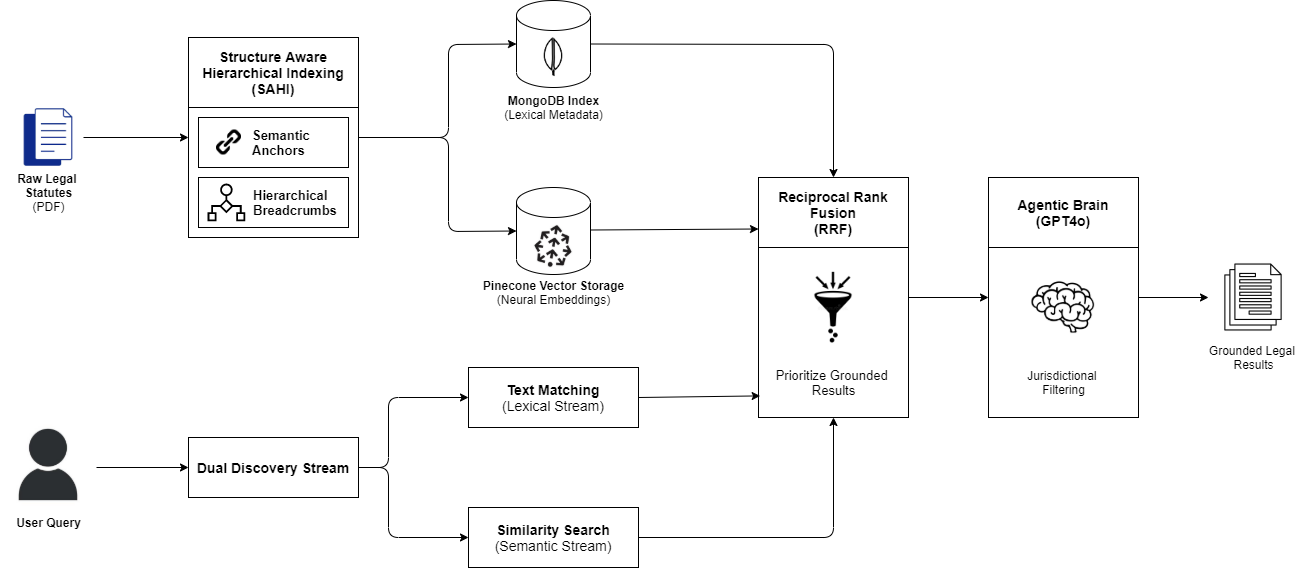
\includegraphics[width=\textwidth]{System Data Flow.png}
    \caption{Agentic RAG Data Pipeline. Raw legal PDFs are processed through SAHI to
    produce semantically anchored, hierarchically tagged text chunks. Dual-Stream
    Discovery retrieves evidence through a Lexical Stream (BM25 over MongoDB) and a
    Semantic Stream (dense vector search over Pinecone) simultaneously. Reciprocal
    Rank Fusion aggregates and re-ranks evidence from both streams. The top-ranked
    evidence is passed to the GPT-4o Agentic Brain for jurisdiction-filtered,
    citation-backed answer generation.}
    \label{fig:dataflow}
\end{figure*}


\subsection{Product Interface}
\label{subsec:product_interface}

Legalyze is a cohesive environment where practitioners can navigate retrieved evidence, audit their drafts for constitutional alignment, and compile an entire case file. This subsection describes the practical modules of the interface and the features that support research efficiency for practitioners. The main benefit of this integrated workflow is that it helps practitioners with demanding schedules. Lawyers can perform all tasks in a single location instead of switching between books, websites, and word processors. This section discusses the different components of the interface and their roles in helping lawyers work more efficiently. This unified approach not only speeds up the research process but also reduces the risk of procedural errors. This subsection explains how these interface modules are structured hierarchically and how they contribute to streamlining professional legal research.

\subsubsection{Chat Interface}

The Legalyze Chat Interface (\autoref{fig:chat}) offers a tri-pane legal natural-language research interface. The left-hand panel contains a chronological list of session history and shortcut buttons to Compliance Checkup and the Case Building Wizard. The central panel houses the conversational AI engine and provides structured legal responses such as document analysis, research, drafting, and case strategy. The right Document Hub panel offers real-time access to professional legal templates, uploaded files, and generated files, enabling a smooth transition between legal research and document creation within a cohesive unit.

\subsubsection{Compliance CheckUp}

A Compliance Checkup (\autoref{fig:compliance}) is an automated process that presents the findings of an audit in a sequentially numbered list of conflicts. Each flagged issue includes a plain-language issue description, a precise Constitutional Basis citing the relevant Part and Article, and an actionable redline containing exact corrective wording to be directly incorporated. Each conflict is accompanied by a collapsible Strategic Reasoning panel, and a concluding section on Compliant Foundations highlights areas of strong constitutional alignment, providing a balanced and not strictly adversarial audit.

\subsubsection{Case Buildup Wizard}

The Case Buildup Wizard (\autoref{fig:wizard}) is a guided, multi-step legal strategy engine designed to take practitioners through a structured workflow of seven stages, presented as a progress pipeline at the top of the interface: Case Intake, Classification, Relevant Law, Precedents, Strategy, Filing Details, and Drafting. In this process, the practitioner is asked to fill in specific case facts and select the positional role of the client, such as Petitioner or Plaintiff, as well as the applicable court level, starting from District and Magistrate courts and moving upward. An interactive ``Start Case Analysis'' button activates the AI engine, while bottom navigation controls allow movement forward or backward through the stages.


\begin{figure*}[p]
\centering
% --- Figure 3 ---
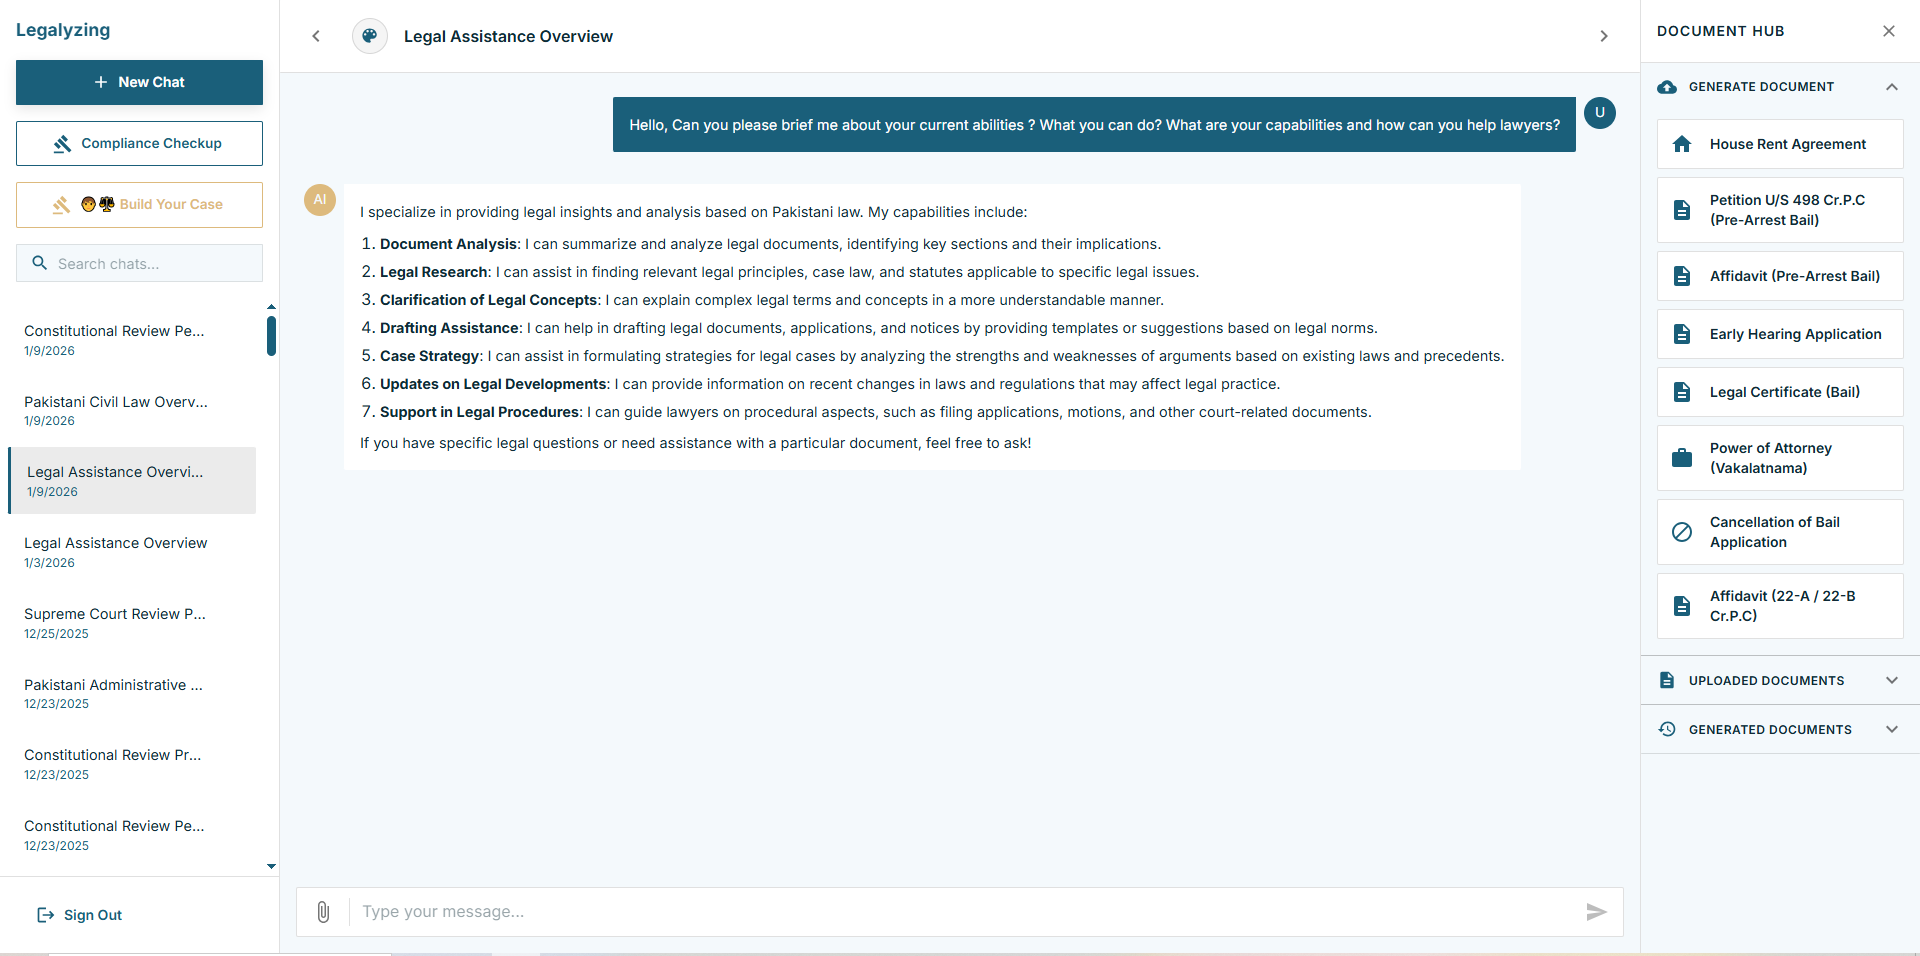
\includegraphics[width=\textwidth]{Legalyze Chat Interface .png}
\caption{The Legalyze Chat Interface provides a unified tri-panel environment for natural-language legal discovery. The left panel maintains a persistent session history of prior consultations, the central panel hosts the conversational AI engine delivering structured legal responses, and the right Document Hub panel offers instant access to professional legal document templates, uploaded documents, and previously generated outputs , bridging legal research and document production within a single workspace.}
\label{fig:chat}

\vspace{1em}

% --- Figure 4 ---
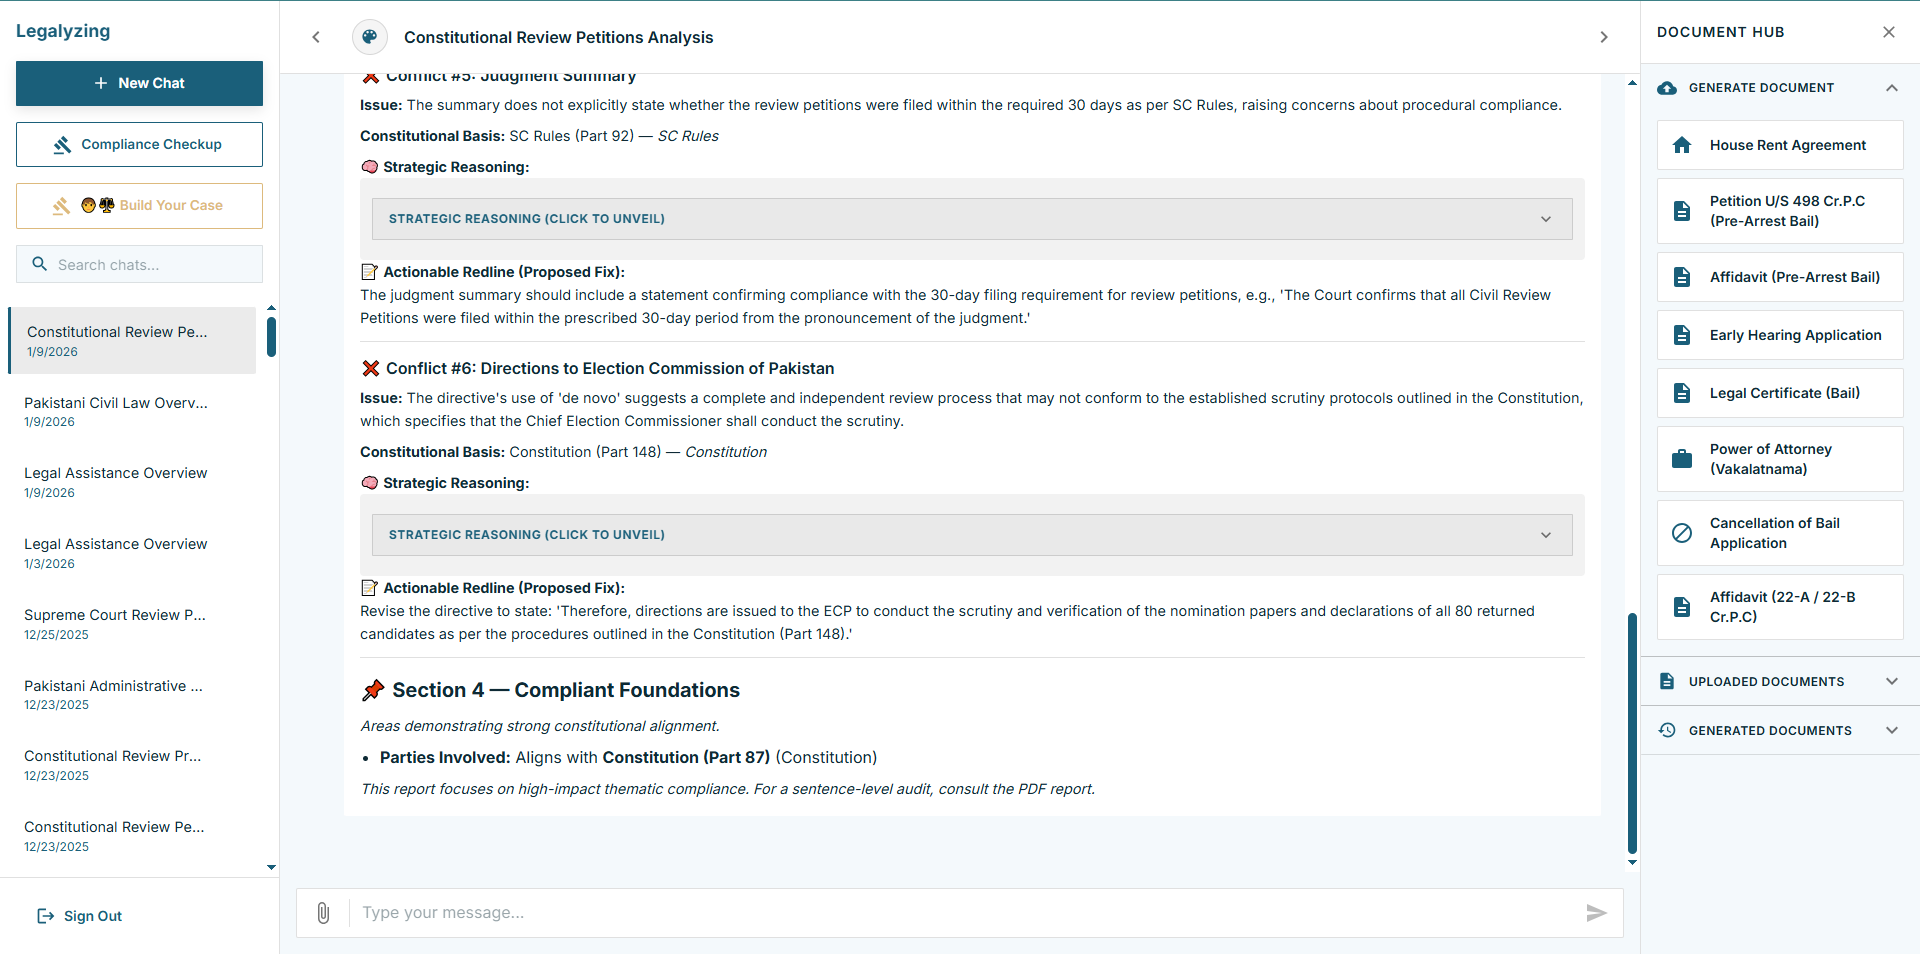
\includegraphics[width=\textwidth]{Compliance CheckUp .png}
\caption{The Compliance CheckUp Module performs automated constitutional auditing of submitted legal manuscripts, flagging each identified conflict with a precise Issue description, a pinpoint Constitutional Basis referencing the applicable Part and Article, and an Actionable Redline proposing verbatim corrective language. }
\label{fig:compliance}
\end{figure*}

\begin{figure*}[p]
\centering
% --- Figure 5 ---
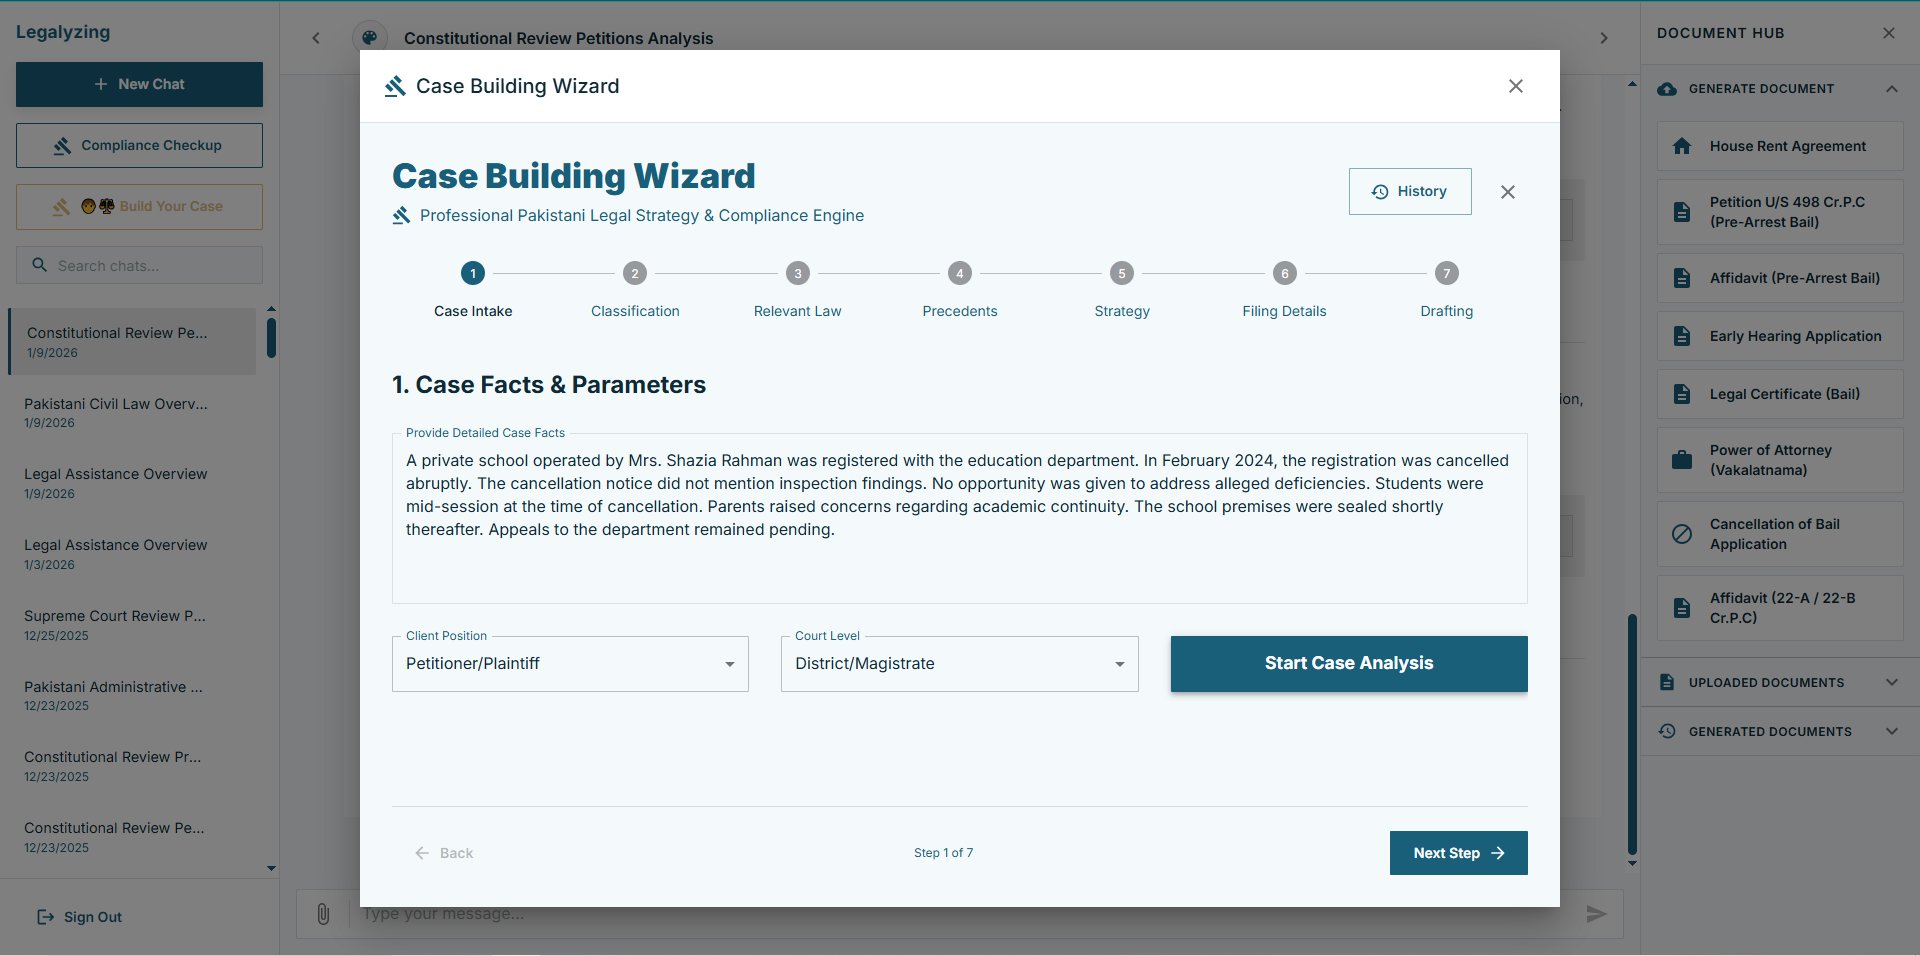
\includegraphics[width=\textwidth]{Case Buildup Wizard.png}
\caption{The Case Building Wizard orchestrates a guided seven-stage legal strategy pipeline , spanning Case Intake, Classification, Relevant Law, Precedents, Strategy, Filing Details, and Drafting. At the Case Intake stage shown, the practitioner enters free-form case facts, selects the client positional role, and specifies the applicable court level before initiating AI-driven analysis, ensuring all jurisdictional and procedural parameters are systematically captured prior to strategy formulation.}
\label{fig:wizard}

\vspace{1em}

% --- Figure 6 ---
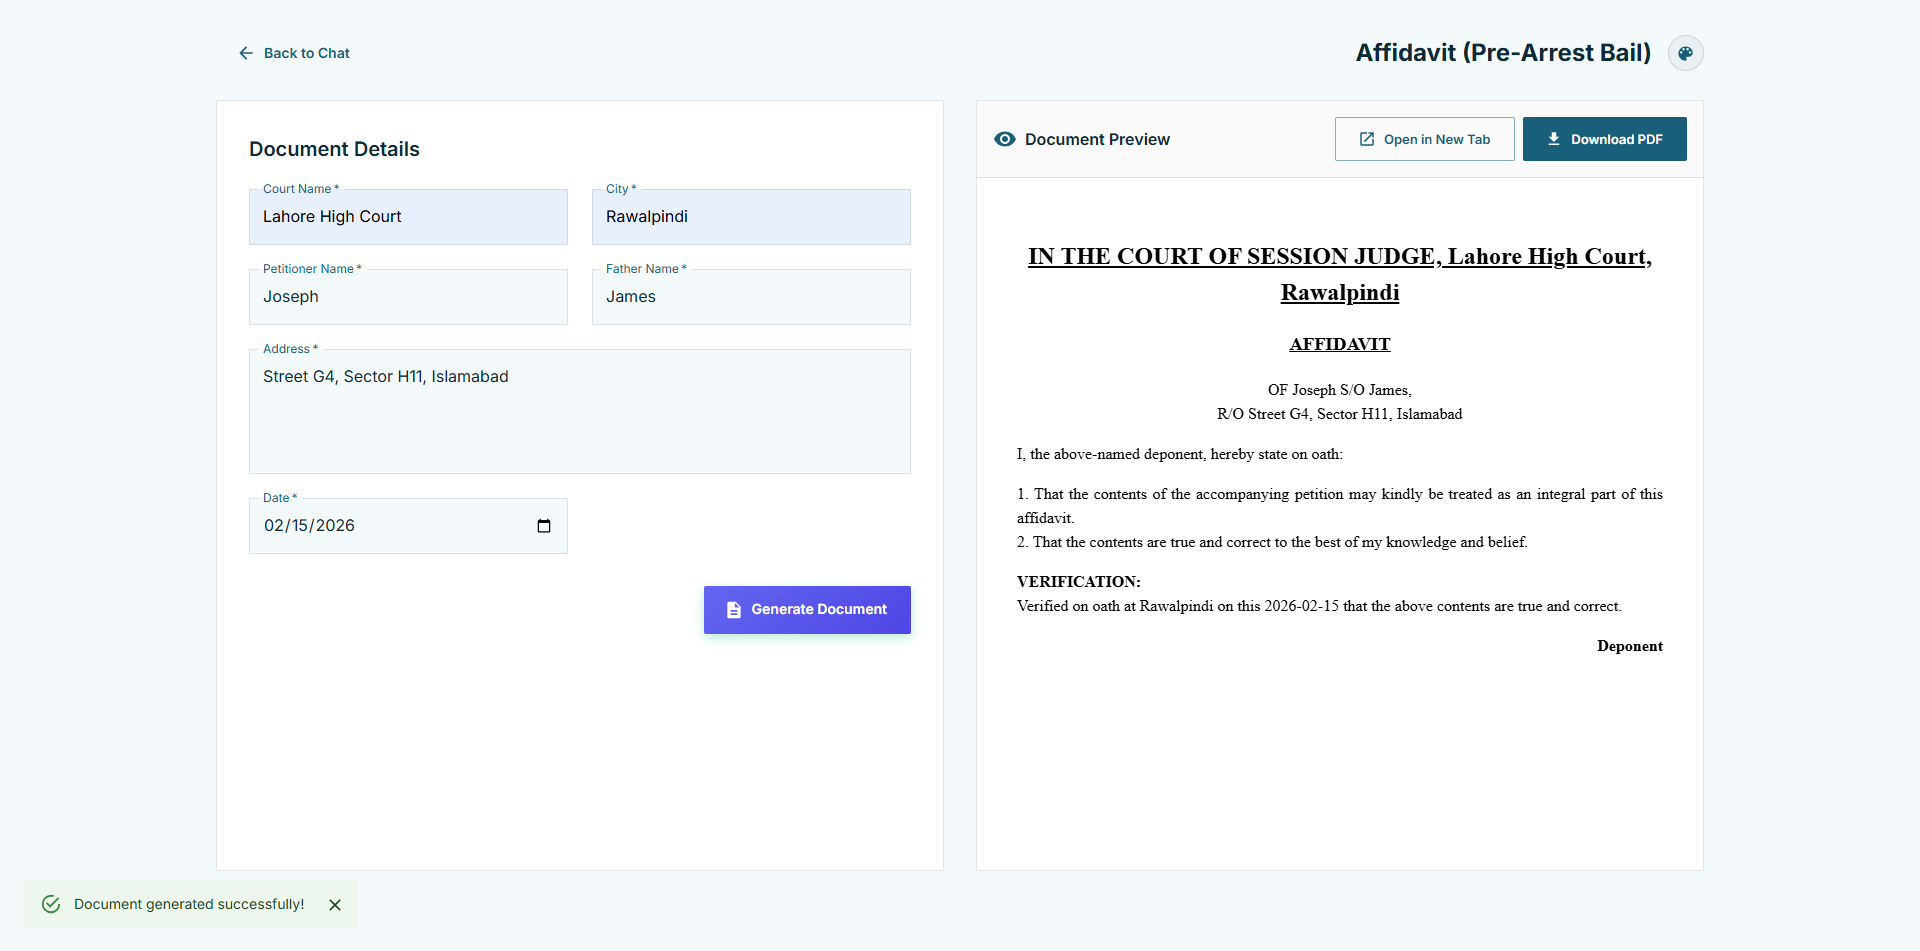
\includegraphics[width=\textwidth]{Document Generation.png}
\caption{The Document Generation Screen provides a split-panel interface for producing court-ready legal documents from jurisdiction-specific templates. The left panel collects structured case metadata (including court name, city, parties, and date ) through clearly labelled input fields, while the right Document Preview panel renders a fully formatted legal document in real time upon generation. }
\label{fig:generation}
\end{figure*}

\subsubsection{Document Generation}

The Document Generation screen (\autoref{fig:generation}) offers a split-screen interface for generating court-ready legal documents based on structured templates with live preview. The left panel displays a Document Details form, which collects all jurisdiction-specific metadata required for the selected template, in this case an Affidavit for Pre-Arrest Bail. It prompts the practitioner to enter details such as Court Name, City, Petitioner Name, Father's Name, residential address, and date into clearly labeled fields. Once the practitioner clicks the Generate Document button, the right panel immediately displays a fully formatted legal document in the preview section. This includes the appropriate legal heading, court designation, declaratory body text, verification clause, and deponent signature block populated with the entered details. The preview panel includes two action buttons in the upper right (Open in New Tab and Download PDF), allowing the practitioner to view the document in full resolution or export it as a submission-ready PDF. A green success notification appears at the bottom of the screen to confirm

\subsection{Analysis}
\label{subsec:analysis}

\rev{Legalyze is analyzed using mathematical models and empirical data. Five Pakistani legal sources were used to build the evaluation corpus (\autoref{fig:corpus}): the Constitution of Pakistan (1973, 280 articles and six schedules), the Pakistan Penal Code (PPC, 1860, 511 sections), the Code of Criminal Procedure (CrPC, 1898), the Qanun-e-Shahadat Order (QSO, 1984, Pakistan's primary evidence statute), and 250 superior court rulings spanning 2018 to 2024. These five sources jointly contain a total of approximately 1.2 million tokens of legal text, with statutory legislation contributing roughly 54\% ($\sim$648,000 tokens) and the case-law collection comprising the remaining 46\% ($\sim$552,000 tokens). To ensure rigorous and comprehensive empirical assessment, the evaluation directly maps these sources into three legal domains: 1)~\textbf{Constitutional Law} (24 queries, 72 reviewer judgments), evaluated against the Constitution of Pakistan (1973); 2)~\textbf{Criminal Law} (23 queries, 69 reviewer judgments), evaluated against the Pakistan Penal Code (PPC, 1860); and 3)~\textbf{Procedural Law} (20 queries, 60 reviewer judgments), evaluated jointly against the Code of Criminal Procedure (CrPC, 1898) for procedural rules and the Qanun-e-Shahadat Order (QSO, 1984) for evidentiary admissibility and burden-of-proof standards. Across all three domains, the 250 superior court judgments provide the contextual judicial interpretation layer and precedent hierarchy. In this subsection, the probabilistic models used to rank evidence and measure similarity are presented, followed by a comparison of hallucination rates across different system configurations. The findings show that structure-aware retrieval is effective in minimizing generated legal errors.}

The retrieval and reliability mechanisms of Legalyze are based on three mathematical
formulations. These equations connect the system architecture to established information
retrieval theory and make the method reproducible and mathematically rigorous. Legalyze
takes the ranked results of the Lexical Stream and Semantic Stream and combines them
using Reciprocal Rank Fusion \cite{r601}. The RRF score of a candidate chunk $d$ is
calculated as follows:

\begin{equation}
  RRF(d) = \sum_{L} \left[ \frac{1}{k + \mathrm{rank}_{L}(d)} \right]
  \label{eq:rrf}
\end{equation}

where $\mathrm{rank}_{L}(d)$ denotes the position of chunk $d$ in ranked list $L$, and
$k = 60$ is a standard smoothing constant. A chunk that appears in both the Lexical and
Semantic streams receives a composite score substantially higher than one appearing in
only one stream. We note that this is an empirical property that in practice
prioritizes consensus candidates on our corpus, and not a mathematical guarantee of
relevance \cite{r601}.

A sentence-embedding model transforms each text chunk and each user query into a
high-dimensional vector representation \cite{r602}. The relevance between a query $q$
and a stored chunk $c$ is measured using cosine similarity:

\begin{equation}
  \mathrm{sim}(q, c) = \frac{\mathbf{v}_{q} \cdot \mathbf{v}_{c}}
                            {\|\mathbf{v}_{q}\|\;\|\mathbf{v}_{c}\|}
  \label{eq:cosine}
\end{equation}

A score of 1.0 indicates that the query and the chunk are semantically identical,
whereas a score near 0 indicates that they are unrelated. Pinecone selects the chunks
with the highest similarity scores to support the Semantic Stream component of the
retrieval pipeline \cite{r603}.

System reliability is quantified using a multi-dimensional legal evaluation framework.
The primary metric is the binary Hallucination Rate (HR), defined as the proportion of
AI-generated legal propositions that qualified expert reviewers cannot trace to any
retrieved or original legal source:

\begin{equation}
  HR = \left( \frac{N_{\text{hallucinated}}}{N_{\text{total}}} \right) \times 100\%
  \label{eq:hr}
\end{equation}

A lower HR indicates a more reliable system. Traceability is determined under a strict
binary criterion: a generated proposition is marked as hallucinated (Y) if and only if
the reviewer cannot locate supporting text in either the retrieved passages or the
original statutory corpus; otherwise it is marked as not hallucinated (N). To provide
a more granular characterisation of legal precision, we define the \textbf{Factual Groundedness vs.\ Legal Accuracy Matrix} (\Cref{tab:matrix}) to distinguish between traceability (hallucination) and accuracy (correctness).

\begin{table}[H]
\caption{\rev{Factual Groundedness vs.\ Legal Accuracy Matrix for Legal AI Evaluation.}
\label{tab:matrix}}
\centering
\small
\begin{tabular}{|l|p{5cm}|p{5cm}|}
\hline
& \textbf{Factual / Correct} & \textbf{Non-Factual / Obsolete} \\ \hline
\textbf{Grounded / Faithful} & \textbf{Category I: Grounded \& Correct} \newline (The retrieved text supports the claim, and the claim is legally correct). & \textbf{Category II: Grounded but Incorrect} \newline (The retrieved text supports the claim, but the text is legally obsolete or misinterpreted). \\ \hline
\textbf{Ungrounded / Unfaithful} & \textbf{Category III: Ungrounded but Correct} \newline (The retrieved text does not support the claim, but the claim is correct based on general LLM memory). & \textbf{Category IV: Ungrounded \& Incorrect} \newline (The retrieved text does not support the claim, and the claim is legally incorrect). \\ \hline
\end{tabular}
\end{table}

This matrix yields two standard metrics:
\begin{equation}
  \text{Faithfulness Rate (FR)} = \left( \frac{\text{Category I} + \text{Category II}}{\text{Total Claims}} \right) \times 100\%
  \label{eq:fr}
\end{equation}
which is related to our primary metric by $HR = 100\% - FR$, and:
\begin{equation}
  \text{Factual Accuracy Rate (FAR)} = \left( \frac{\text{Category I} + \text{Category III}}{\text{Total Claims}} \right) \times 100\%
  \label{eq:far}
\end{equation}
Additionally, we define:
\begin{itemize}
  \item \textbf{Answer Correctness (AC):} Equivalent to FAR, the proportion of generated responses that are factually and legally accurate according to the statutory corpus.
  \item \textbf{Citation Precision (CP):} The proportion of cited legal sources that directly entail the associated generated assertion.
  \item \textbf{Citation Recall (CR):} The proportion of all relevant statutory provisions for a given query that are successfully cited in the generated response.
\end{itemize}

Empirical results for the primary HR metric are reported in \Cref{sec:results}. AC, CP,
and CR are introduced here to provide a complete multi-dimensional evaluation vocabulary
for future comparative studies; their full empirical measurement is deferred to
subsequent work that incorporates a larger annotated benchmark.

Furthermore, to resolve precedent conflicts during context synthesis (such as when two High Courts issue conflicting rulings on the same statutory provision), the system
implements an adjudication protocol following Article~189 of the Constitution of
Pakistan (1973), which dictates that decisions of the Supreme Court of Pakistan are
binding on all other courts. In cases of conflicting High Court precedents, the system
applies hierarchical weighting: Supreme Court rulings (Article~189) take priority over
High Court rulings (Article~201), and larger benches take priority over single-judge
benches \cite{r605}.

\subsection{Experimental Setup}
\label{subsec:setup}

\rev{The hallucination study was conducted on \textbf{67 legal queries} drawn from three legal domains: Constitutional Law (24 queries, 35.8\%, targeting the Constitution of Pakistan), Criminal Law/PPC (23 queries, 34.3\%, targeting the Pakistan Penal Code), and Procedural Law (20 queries, 29.9\%, jointly drawing upon the Code of Criminal Procedure [CrPC] for procedural rules and the Qanun-e-Shahadat Order [QSO] for evidentiary admissibility standards, with the 250 superior court judgments providing contextual judicial interpretation across all three domains). Each query was executed on all three systems, yielding 201 generated responses ($67 \times 3 = 201$). Each response received a single binary traceability label from each reviewer, yielding 201 individual judgments per configuration and 603 judgments in total. The same 67 queries were used across all three configurations to ensure a paired and directly comparable design.} The
Zero-Shot GPT-4o baseline establishes the parametric capability of the underlying
language model without any external retrieval, isolating the model's inherent rate of
legal hallucination when relying solely on pre-trained weights. The Standard RAG (flat
chunking without SAHI) baseline directly isolates the performance impact of our proposed
Structure-Aware Hierarchical Indexing and dual-stream pipeline by holding all other
factors constant. Commercial proprietary systems (e.g., Harvey AI, Westlaw Precision)
were excluded because they do not support the Pakistani legal jurisdiction and do not
provide API access for comparative evaluation. Open-source legal systems trained for
other jurisdictions (e.g., ChatLaw for Chinese law) are structurally incompatible with
the English/Urdu statutory framework of Pakistan.

\rev{Three independent qualified legal reviewers, active Advocates of the High Court of Pakistan each with between five and eight years of litigation experience in Pakistan's superior courts, assessed all 201 responses under a \textbf{reviewer-blinded evaluation
protocol}\footnote{The term ``blinded'' is used in the sense that reviewers were blinded
to the identity of the source system; the research team necessarily knew which
configuration generated each response. This follows standard practice for human-subject
evaluation studies.}: reviewers saw only the query, the retrieved source passage (if
any), and the generated response. For Zero-Shot responses, reviewers were shown the
placeholder text \emph{``(No retrieval passage: this response was generated without source context.)''}. The system identity mapping (System A/B/C) was decoded only after
all reviews were complete. Reviewers independently annotated each response using the
binary traceability criterion: a response is marked as hallucinated (N) if the reviewer
cannot locate supporting text in either the retrieved passages or the original statutory
corpus; otherwise it is marked as traceable (Y). In a subsequent joint session, any
disagreements were resolved by majority discussion to produce a single consensus label
per response, yielding two datasets: a \textbf{pooled dataset} of 201 individual
judgments per configuration and a \textbf{consensus-adjudicated dataset} of 67 unique
response labels per configuration.}
Both datasets are reported in \Cref{sec:results} to ensure complete methodological
transparency.

\rev{To evaluate the empirical findings with statistical rigor, four complementary inferential methods are employed:
\begin{enumerate}
  \item \textbf{Inter-Rater Reliability (Fleiss' Kappa, $\kappa$)} is calculated across the three independent legal reviewers within each system configuration to quantify multi-rater agreement on the binary traceability criteria.
  \item \textbf{Omnibus Paired Hypothesis Testing (Cochran's $Q$ Test)} is conducted on the $N = 67$ paired, repeated-measures consensus judgments across the three system configurations (Zero-Shot, Standard RAG, and Legalyze) to establish whether overall differences in hallucination rates are statistically significant without violating observational independence.
  \item \textbf{Pairwise Contrasts (Exact Binomial McNemar Tests)} are applied to each paired $2 \times 2$ system contingency table, calculating exact two-tailed $p$-values to evaluate the statistical significance of pairwise reductions in legal hallucinations.
  \item \textbf{Clustered Binary Regression (Generalized Estimating Equations - GEE)} is fitted on the full pooled dataset ($N = 603$ total judgments) using a binomial logit link, exchangeable working correlation structure, and robust Huber-White sandwich standard errors to estimate adjusted odds ratios (OR) and confidence intervals while formally accounting for within-query repeated-measures clustering across reviewers.
\end{enumerate}}



\section{Results}
\label{sec:results}
This section presents the experimental results of the Legalyze platform following the
evaluation. The data is assessed based on the system performance measures outlined in
\Cref{subsec:analysis} to show improvements in retrieval accuracy and the reduction in
hallucinations. These findings affirm the usefulness of structure-aware architectures in
achieving reliability in high-stakes legal contexts.

The frequency of legally ungrounded claims generated by each system configuration is
reported in \Cref{tab:hr} and \autoref{fig:hr}. \rev{A total of \textbf{201 generated responses} (67 legal queries $\times$ 3 system configurations) were assessed by three
independent qualified legal reviewers under a reviewer-blinded evaluation protocol, as
described in \Cref{subsec:setup}. Each response received a single binary traceability
label from each reviewer.}

\begin{figure}[H]
\centering
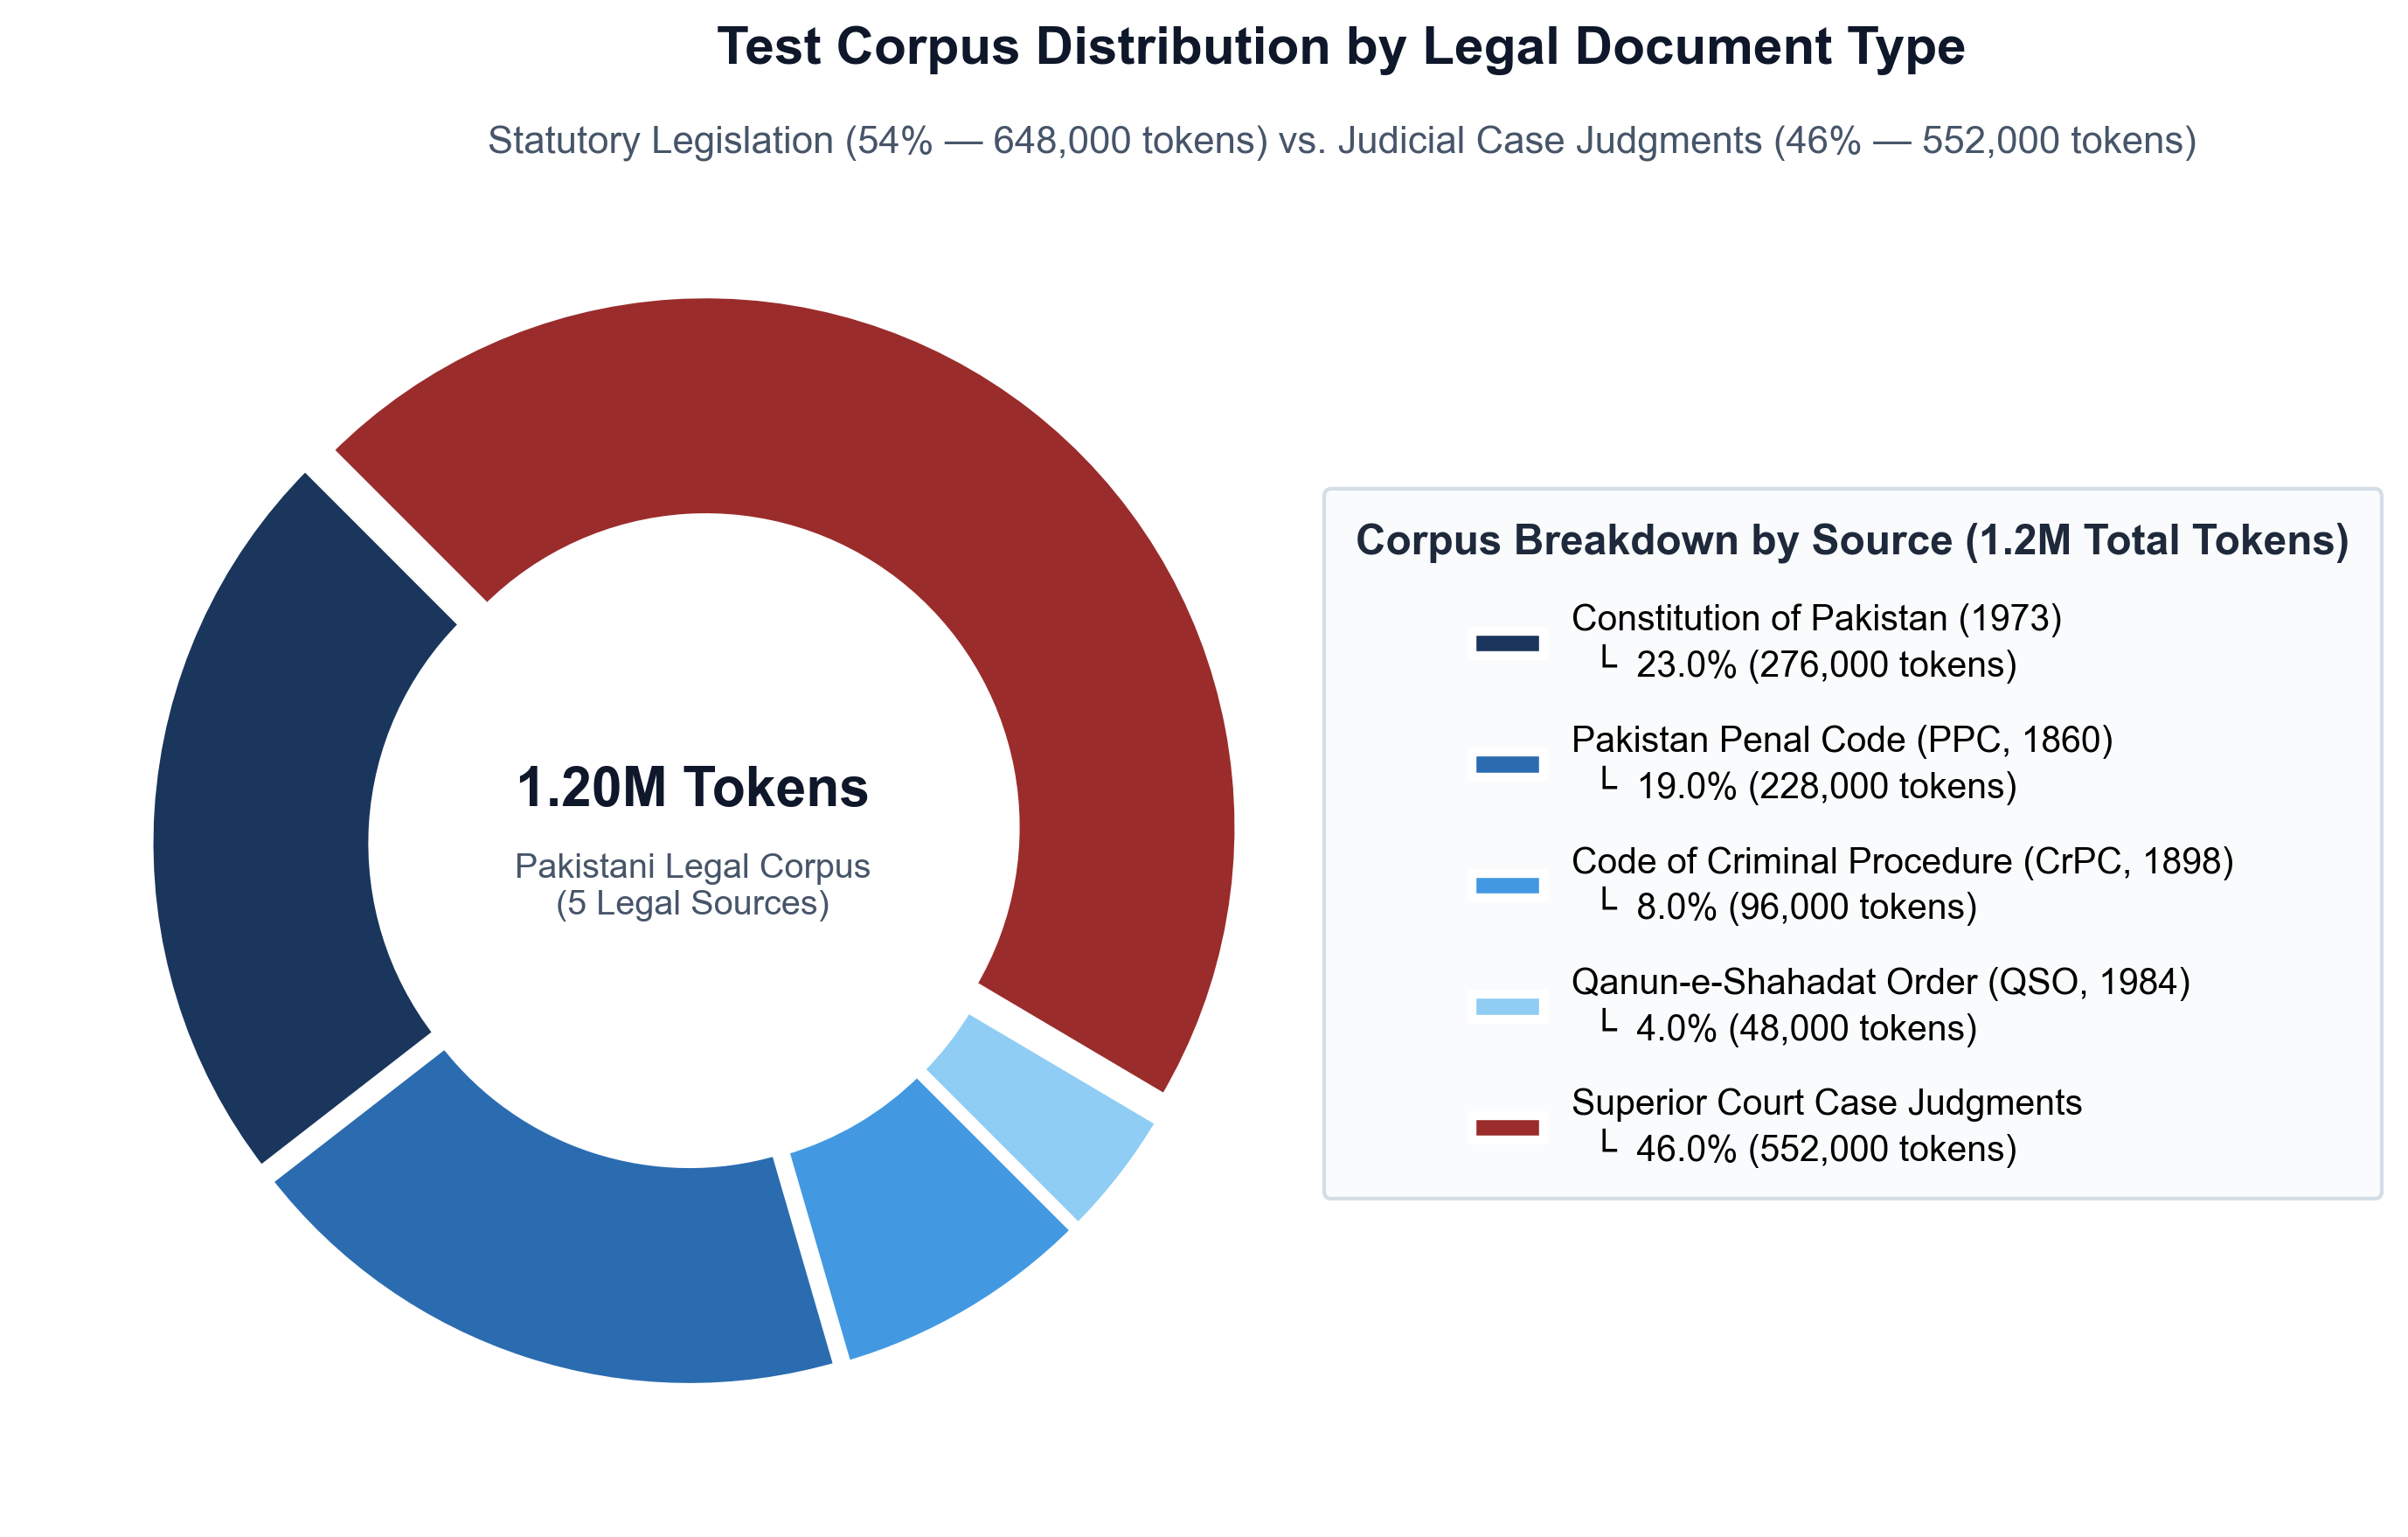
\includegraphics[width=0.55\linewidth]{Test Corpus Distribution by Document Type.png}
\caption{\rev{Test Corpus Distribution by Document Type. The evaluation corpus consists
of approximately 1.2 million tokens drawn from five Pakistani legal sources: Constitution
of Pakistan, PPC, CrPC, Qanun-e-Shahadat Order, and 250 superior court judgments.
Constitutional statutes account for roughly 54\% and the case-law collection for the
remaining 46\%.}}
\label{fig:corpus}
\end{figure}

\begin{figure}[H]
\centering
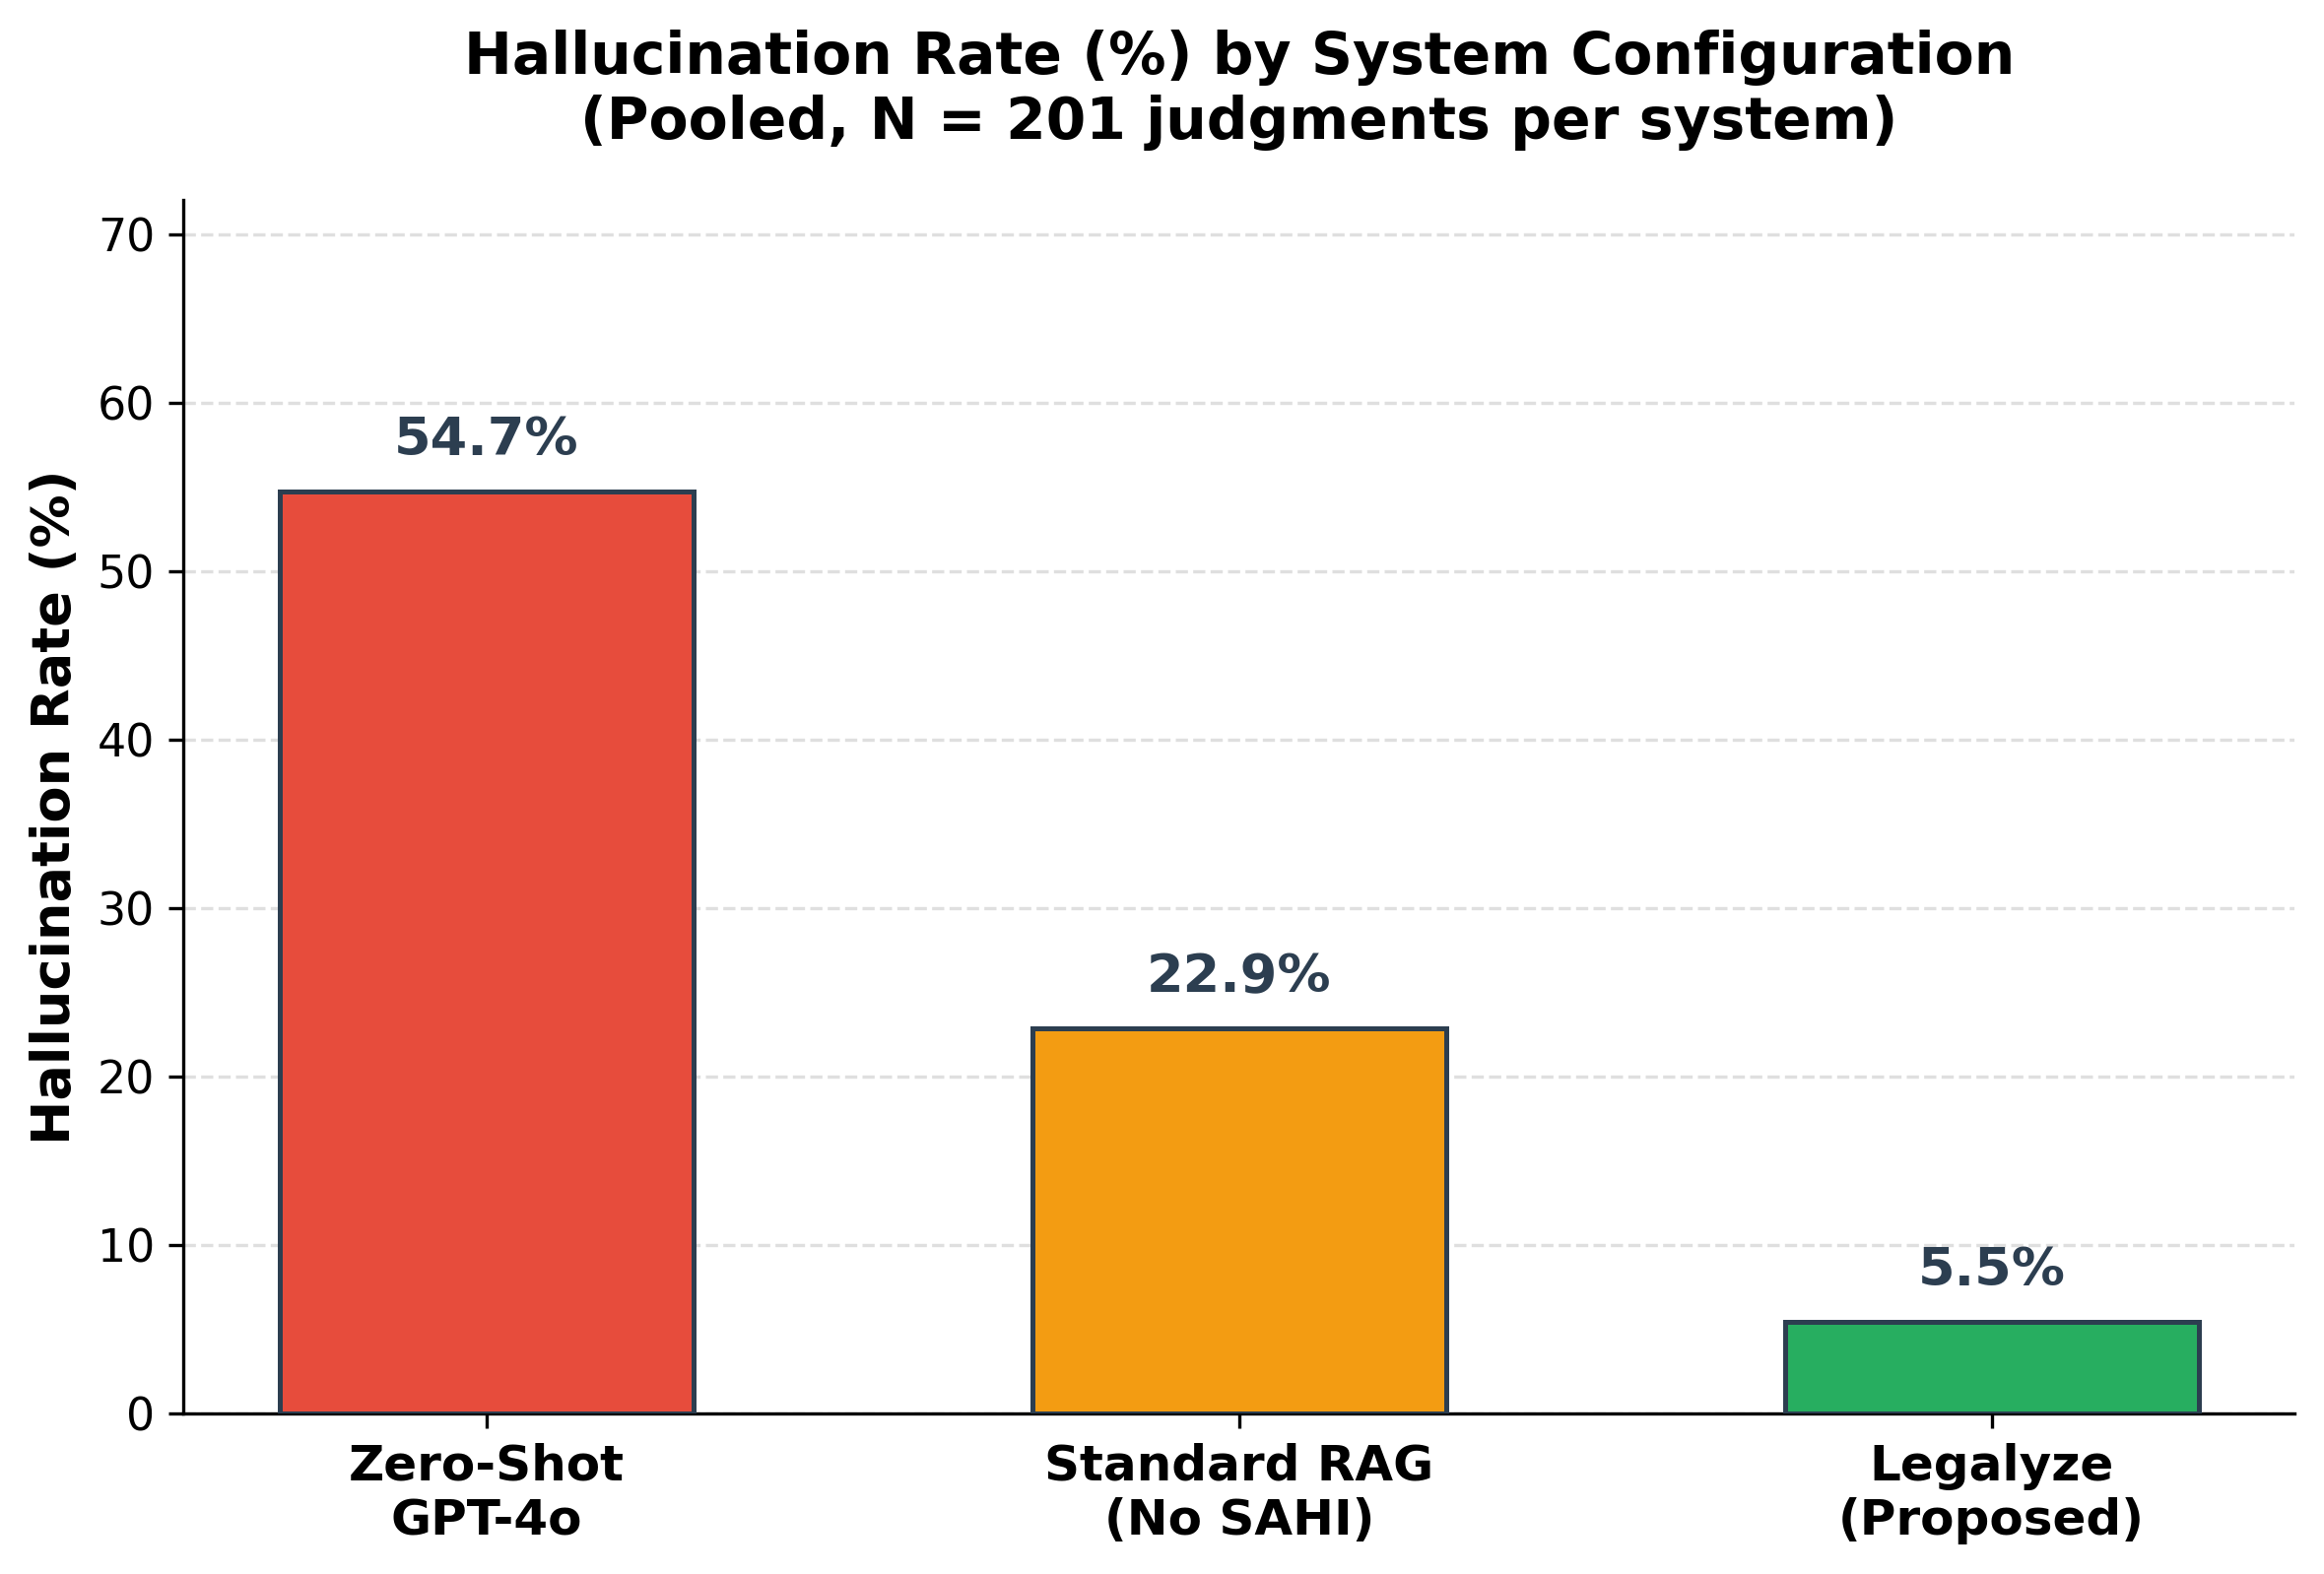
\includegraphics[width=0.55\linewidth]{HR Image.png}
\caption{Hallucination Rate (\%) by System Configuration. Legalyze achieves a
substantial reduction in hallucination compared to the zero-shot baseline, decreasing
the overall pooled HR from 54.7\% to 5.5\% across evaluated legal domains.}
\label{fig:hr}
\end{figure}
\begin{table}[H]
\caption{\rev{Hallucination Rate (HR\%) by system configuration and legal domain
(Pooled, $N = 201$ judgments per system; consensus-adjudicated, $N = 67$ unique
response labels per system).}}
\label{tab:hr}
\centering
\small
\begin{tabularx}{\textwidth}{|X|c|c|c|c|}
\hline
\textbf{System Configuration} & \textbf{Const.\ HR\% (N=72)} & \textbf{Crim.\ HR\% (N=69)}
  & \textbf{Proc.\ (CrPC/QSO) HR\% (N=60)} & \textbf{Overall HR\% (N=201)} \\ \hline
Zero-Shot GPT-4o (No Retrieval)              & 54.2\% (39/72) & 60.9\% (42/69) & 48.3\% (29/60) & 54.7\% (110/201) \\ \hline
Standard RAG without SAHI Indexing           & 22.2\% (16/72) & 26.1\% (18/69) & 20.0\% (12/60) & 22.9\% (46/201)  \\ \hline
\rev{Offline SAHI Hybrid with RRF}            & 5.6\% (4/72)   & 5.8\% (4/69)   & 5.0\% (3/60)   & 5.5\% (11/201)   \\ \hline
\end{tabularx}
\end{table}



The overall incidence of hallucinations decreases from 54.7\% with no retrieval, to
22.9\% for the standard RAG system, and further to 5.5\% for the full Legalyze system.
Using \cref{eq:hr}, this corresponds to a 90.0\% relative reduction over the zero-shot
baseline. The improvement is consistent across all three legal sub-domains. Notably, the
largest gains are observed in criminal law, where statutory precision is most critical
and where general-purpose models tend to confuse semantically similar but legally
distinct statutory provisions. The procedural domain also benefits from the hierarchical tagging
of SAHI, as procedural rules are highly structured across court levels and jurisdictional
hierarchies that are often overlooked by flat retrieval systems. Together, these results
confirm that the performance advantage of Legalyze is not limited to a specific area of
law but is a systematic and consistent outcome of its structure-aware design, \rev{providing encouraging empirical evidence for its potential as a legal research and decision-support aid under human expert verification.}

To illustrate how the architectural differences between configurations translate qualitatively into response output and hallucination behavior, \Cref{tab:sample_comparison} provides a comparative analysis of a single representative query execution across the three configurations.

\begin{table*}[t]
\caption{Qualitative Comparison of Query Execution across Zero-Shot, Standard RAG, and Legalyze (Query ST-032).}
\label{tab:sample_comparison}
\centering
\small
\begin{tabularx}{\textwidth}{|l|>{\raggedright\arraybackslash\hsize=1.1\hsize}X|>{\raggedright\arraybackslash\hsize=1.1\hsize}X|>{\raggedright\arraybackslash\hsize=0.8\hsize}X|}
\hline
\textbf{Configuration} & \textbf{Retrieved Source Passage} & \textbf{Generated Response} & \textbf{Reviewer Evaluation} \\ \hline
\multicolumn{4}{|l|}{\textbf{Query (ST-032):} How does extortion under Section 383 PPC differ from theft under Section 378 PPC?} \\ \hline
\textbf{Zero-Shot} & 
\emph{No retrieval was used for this configuration.} & 
Extortion under Section 383 of the Pakistan Penal Code (PPC) differs from theft under Section 378 PPC. Extortion involves intentionally putting a person in fear of injury and thereby inducing them to deliver property. Theft, on the other hand, involves dishonestly taking movable property out of the possession of another person without their consent. & 
\textbf{N / Hallucinated} \newline (Unverified in context; no retrieved passage provided) \\ \hline
\textbf{Standard RAG} & 
\texttt{[Pakistan Penal Code, Section 379] Punishment for theft:} Whoever commits theft shall be punished with imprisonment of either description for a term which may extend to three years, or with fine, or with both. & 
Extortion under Section 383 PPC differs from theft under Section 378 PPC. According to Section 379, theft is punished with up to three years of imprisonment. Extortion under Section 383 PPC is when a person is put in fear of injury to deliver property, which is punished under Section 384 PPC with up to three years of imprisonment. & 
\textbf{N / Hallucinated} \newline (The response references Section 383 and 384, which are not present in retrieved Section 379) \\ \hline
\textbf{Legalyze} & 
\texttt{[Pakistan Penal Code, Section 378] Theft:} Whoever, intending to take dishonestly any moveable property out of the possession of any person without that person's consent, moves that property... \newline
\texttt{[Pakistan Penal Code, Section 383] Extortion:} Whoever intentionally puts any person in fear of any injury... and thereby dishonestly induces the person so put in fear to deliver... any property... & 
Under the Pakistan Penal Code (PPC), theft (Section 378) and extortion (Section 383) are distinguished by consent and coercion: 1) Theft involves taking moveable property out of someone's possession without their consent (Section 378). 2) Extortion involves inducing a person to deliver property by putting them in fear of injury (Section 383). & 
\textbf{Y / Traceable} \newline (Every claim is directly traceable to the retrieved source passages for Section 378 and 383) \\ \hline
\end{tabularx}
\end{table*}

\rev{Three independent qualified legal reviewers, active Advocates of the High Court of Pakistan with between five and eight years of litigation experience in Pakistan's superior courts, assessed all 201 responses. In the pooled analysis, each of the 67 responses was independently evaluated by all three reviewers, resulting in $N = 201$ total individual judgments per configuration (603 total judgments across all three configurations). These pooled judgments underlie the overall hallucination rates reported in \cref{tab:hr} (where 11 out of 201 judgments for Legalyze yields 5.5\%, and 46 out of 201 for Standard RAG yields 22.9\%). In addition, reviewers conducted a joint consensus adjudication session where disagreements were resolved by majority discussion, producing a consensus-adjudicated dataset of $N = 67$ unique response classifications, yielding overall consensus rates of 55.2\% for Zero-Shot, 23.9\% for Standard RAG, and 4.5\% for Legalyze. Reporting both datasets ensures complete transparency and resolves the mathematical increment properties of the overall percentages.}

\rev{To measure the reliability of these evaluations, Fleiss' Kappa ($\kappa$) was computed
across the three reviewers within each configuration, yielding $\kappa = 0.659$ for
Zero-Shot, $\kappa = 0.718$ for Standard RAG, and $\kappa = 0.615$ for Legalyze,
with an overall Fleiss' Kappa of $\kappa = 0.743$. Per the Landis \& Koch (1977)
scale, values above 0.60 represent \textbf{substantial agreement}, confirming that
the evaluation is reproducible and that the reported hallucination rates reflect a
genuine and consistent consensus among independent qualified reviewers.}

\subsection{End-to-End Hallucination Evaluation}

The paired experimental design, where the identical 67 queries were executed across all three systems, requires statistical tests that account for the repeated-measures structure.
We therefore report Cochran's Q test on the consensus-adjudicated dataset and pairwise
McNemar tests as post-hoc comparisons, followed by a Generalized Estimating Equations
(GEE) analysis on the pooled reviewer judgments to account for clustering by query.

\rev{\textbf{Cochran's Q Test} (consensus-adjudicated dataset, $N = 67$ queries):
$Q = 37.57$, $df = 2$, $p = 6.93 \times 10^{-9}$ (extremely significant across all
three configurations simultaneously).}

\rev{\textbf{Pairwise McNemar Tests} (exact binomial; all pairwise comparisons statistically significant):}
\begin{enumerate}
  \item \rev{Zero-Shot vs.\ Standard RAG: $p = 7.53 \times 10^{-4}$}
  \item \rev{Zero-Shot vs.\ Legalyze: $p = 5.40 \times 10^{-9}$}
  \item \rev{Standard RAG vs.\ Legalyze: $p = 4.43 \times 10^{-3}$}
\end{enumerate}

\rev{\textbf{GEE Analysis} (pooled, $N = 603$ judgments, 67 query clusters, Binomial
family, exchangeable within-query correlation, robust sandwich SE;
reference category = Legalyze):}
\begin{enumerate}
  \item \rev{Standard RAG vs.\ Legalyze: OR $= 5.13$ [95\% CI: 1.76, 14.92], $p = 0.003$}
  \item \rev{Zero-Shot vs.\ Legalyze: OR $= 20.88$ [95\% CI: 7.29, 59.81], $p = 1.52 \times 10^{-8}$}
\end{enumerate}
\rev{The GEE results confirm that, after accounting for repeated measurements across the
same 67 queries, Standard RAG has 5.1$\times$ higher odds of hallucination than
Legalyze, and Zero-Shot has 20.9$\times$ higher odds; both are highly statistically
significant.}

\rev{\textbf{95\% Wilson Confidence Intervals} (consensus-adjudicated, $N = 67$):
Zero-Shot: 55.2\% [43.4\%, 66.5\%]; Standard RAG: 23.9\% [15.3\%, 35.3\%];
Legalyze: 4.5\% [1.5\%, 12.4\%].}

\rev{\textbf{Note on Fleiss' Kappa.} Per-configuration Fleiss' $\kappa$ values (Zero-Shot:
$\kappa = 0.659$; Standard RAG: $\kappa = 0.718$; Legalyze: $\kappa = 0.615$) are
lower than the overall pooled $\kappa = 0.743$. This is a well-documented statistical
phenomenon known as the \emph{prevalence effect} (Feinstein \& Cicchetti, 1990):
when one category dominates within a single configuration (e.g., 94.5\% ``Y'' for
Legalyze), expected agreement by chance ($P_e$) is very high, which deflates the
per-configuration $\kappa$. Pooling all three configurations produces a more balanced
Y/N distribution, which reduces $P_e$ and yields a higher overall $\kappa$. This is
not an inconsistency; it is an inherent mathematical property of $\kappa$ under
skewed distributions and does not affect the reliability interpretation.}

\subsection{SAHI Parser Accuracy Evaluation}

The core component of Legalyze is the SAHI parser. To evaluate its technical precision,
we tested its execution against a manually verified ground-truth set of 56 constitutional
articles representing all 12 parts of the Constitution of Pakistan (451~KB, 6,346
lines). The parser achieved:
\begin{itemize}
  \item \textbf{Article Detection Rate:} 64.3\% (36 out of 56 ground-truth articles
  successfully isolated and chunked). Missed detections were primarily caused by complex
  sub-number suffixes (e.g., Articles 10A, 25A, 63A) and OCR text artifacts.
  \item \textbf{Part Assignment Accuracy:} 55.6\% (20 out of 36 detected articles
  correctly associated with their parent Part headers).
  \item \textbf{Overall Parsing Accuracy:} 35.7\% (20 out of 56 articles with fully
  correct structural annotations).
\end{itemize}
This empirical baseline highlights a structural drift limitation in rule-based parsing
of poorly formatted legal texts, representing an area for future improvement using
LLM-assisted section classification.

To explain how the system maintains high retrieval and hallucination reduction
performance despite this modest parsing accuracy, it is critical to note three architectural
factors:
\begin{enumerate}
  \item \textbf{Hierarchy vs.\ Item Granularity:} The parser evaluation measures the \emph{exact} path matching (e.g., matching every nested Part, Chapter, and Article correctly). However, end-to-end retrieval is resilient to partial path errors; matching even a single structural level (e.g., the article number itself, such as Article~12, even if the parent Chapter is misidentified due to nested OCR lines) is sufficient to isolate the correct target region and exclude other irrelevant statutes.
  \item \textbf{Redundancy in Search Channels:} The dual-stream pipeline retrieves chunks via separate dense and lexical channels. If a parsing error leads to an incorrect structural annotation, the lexical keyword matching stream (e.g., matching the phrase ``double jeopardy'' in Article~12) still retrieves the target chunk. Reciprocal Rank Fusion (RRF) then resolves rank discrepancies, ensuring that individual metadata extraction errors do not act as single points of failure.
  \item \textbf{Preservation of Vector Space Similarity:} An article-level chunk with incorrect parent metadata annotations still contains the correct raw text body. The semantic embeddings are derived from this text, keeping the vector-space similarity calculation unaffected. SAHI's structural annotations act as a soft boosting signal rather than a hard constraint, ensuring that the system benefits from structure-aware chunk boundaries even when the parser fails to reconstruct the absolute hierarchy path.
\end{enumerate}
This structural redundancy and rank-level resilience explain why Legalyze yields a 90.0\% relative reduction in hallucinations (5.5\% vs.\ 54.7\% baseline) despite the rule-based parser's modest 35.7\% overall accuracy.


\subsection{Retrieval Ablation Study}

To isolate retrieval behaviour independently of generation, we conducted a local offline
retrieval evaluation on 20 manually curated legal queries. \rev{In this offline study,
the dense retrieval stream is approximated by a character 3-gram vector space model
(VSM) rather than the production Pinecone sentence-embedding model, which constitutes
a conservative local proxy. Full online evaluation with the production embedding model
is planned as future work.} To isolate the contributions of SAHI, hybrid search, and
RRF, seven configurations were evaluated:
\begin{enumerate}
  \item \textbf{Flat Lexical Only:} Word-level BM25 indexing over fixed-window chunks.
  \item \textbf{Flat Dense Only:} Cosine similarity over character 3-gram VSM embeddings
  of fixed-window chunks, serving as a deterministic local proxy for vector-space
  similarity.
  \item \textbf{Flat Hybrid (Score Sum):} Standard score-based hybrid retrieval combining
  normalized BM25 and VSM dense scores via a linear combination ($0.5 \times S_{\text{norm, Lex}} + 0.5 \times S_{\text{norm, Dense}}$).
  \item \textbf{Flat Hybrid (RRF):} Combined flat lexical and VSM dense retrieval fused
  via RRF, representing standard hybrid retrieval without structure-aware indexing.
  \item \textbf{SAHI Lexical Only:} BM25 indexing over structure-aware article-level
  chunks.
  \item \textbf{SAHI Dense Only:} Cosine similarity over structure-aware article-level
  chunk VSM embeddings.
  \item \textbf{Offline SAHI Hybrid with RRF\textsuperscript{$\dagger$} (Proposed):} Structure-aware chunks with fused lexical
  and VSM dense streams via RRF.
\end{enumerate}

Retrieval performance is measured using Recall@5, Recall@10, Precision@5, Mean
Reciprocal Rank (MRR), and Normalized Discounted Cumulative Gain (nDCG@10). Results
are presented in \Cref{tab:ablation}.

\begin{table}[H]
\caption{\rev{Retrieval Ablation Results across seven configurations (20 ground-truth
queries). $\dagger$ All configurations use character 3-gram cosine similarity as the
dense retrieval proxy; the deployed production system uses Pinecone sentence embeddings.
These results therefore characterise the offline surrogate pipeline.}}
\label{tab:ablation}
\centering
\small
\begin{tabular}{lcccccc}
\hline
\textbf{Configuration} & \textbf{R@5} & \textbf{R@10} & \textbf{P@5}
  & \textbf{MRR} & \textbf{nDCG@5} & \textbf{nDCG@10} \\ \hline
Flat Lexical Only       & 45.0\% & 50.0\% &  9.0\% & 0.384 & 0.394 & 0.411 \\
Flat Dense Only         & 35.0\% & 45.0\% &  7.0\% & 0.281 & 0.288 & 0.322 \\
Flat Hybrid (Score Sum) & 45.0\% & 50.0\% &  9.0\% & 0.384 & 0.397 & 0.411 \\
Flat Hybrid (RRF)       & 40.0\% & 50.0\% &  8.0\% & 0.413 & 0.400 & 0.432 \\
SAHI Lexical Only       & 55.0\% & 60.0\% & 11.0\% & 0.532 & 0.532 & 0.548 \\
SAHI Dense Only         & 60.0\% & 65.0\% & 12.0\% & 0.525 & 0.538 & 0.556 \\
\textbf{SAHI Hybrid + RRF$^\dagger$}  & \textbf{65.0\%} & \textbf{65.0\%} & \textbf{13.0\%}
  & \textbf{0.477} & \textbf{0.519} & \textbf{0.519} \\ \hline
\end{tabular}
\end{table}

The ablation study demonstrates that incorporating structural metadata (SAHI) yields the largest performance increase, elevating dense Recall@5 from 35.0\% to 60.0\% and lexical Recall@5 from 45.0\% to 55.0\%. Comparing Flat Hybrid (Score Sum) with Flat Hybrid (RRF) reveals a distinct trade-off: standard score normalization maintains similar recall but suffers from lower top-rank precision (MRR 0.384 vs.\ 0.413 for RRF), validating RRF's rank-level robustness under rank disagreement. \rev{Combining the SAHI streams under the offline SAHI Hybrid with RRF configuration achieves the highest Recall@5 of 65.0\%. A small reduction in MRR (0.477) for the offline SAHI Hybrid with RRF configuration compared to SAHI Dense Only (MRR 0.525) is observed, highlighting that while RRF broadens overall recall coverage, it can occasionally penalize the absolute rank order of the single highest-confidence stream.}

\subsection{Hallucination Rate Domain Analysis}

The overall hallucination rate decreases from 54.7\% with no retrieval, to 22.9\% with
standard RAG, and further to 5.5\% with the full Legalyze system. Using \cref{eq:hr},
this corresponds to a 90.0\% relative reduction over the zero-shot baseline, consistent
across all three legal sub-domains (as shown in \Cref{tab:hr}). The largest gains are
observed in criminal law, where statutory precision is most critical and where
general-purpose models tend to confuse semantically similar but legally distinct
provisions. The procedural domain also benefits substantially from SAHI's hierarchical
tagging, because procedural rules are highly structured across court levels and
jurisdictional hierarchies that flat retrieval systems routinely overlook. Together,
these results confirm that the performance advantage of Legalyze is not domain-specific
but a systematic outcome of its structure-aware design.


\section{Discussion}
\label{sec:discussion}

\hspace*{2em}In this research, a verifiable expert system designed to address the
reliability gap in the Pakistani legal ecosystem is introduced by providing
structure-aware, verifiable intelligence, called Legalyze \cite{r605}. Recent empirical
audits show that hallucinations in legal AI systems can occur at rates of up to 58\%,
highlighting the severity of the reliability gap \cite{r40}. This section discusses the
experimental results and compares the performance of Legalyze with other state-of-the-art
retrieval-augmented solutions \cite{r40,r45}. The discussion highlights how the risks of
hallucination, which currently limit the application of AI in high-stakes legal contexts,
can be mitigated through careful architectural design.

\hspace*{2em}The measured 90.0\% relative decrease in hallucination rates, falling from a 54.7\% pooled baseline in zero-shot models to 5.5\% in the Legalyze framework, suggests
that in our experiments, the accuracy of the grounding mechanism, rather than the raw
reasoning ability of the language model, was a critical bottleneck in legal AI. This is
especially clear in conventional RAG systems, where flat chunking does not preserve
statutory context and jurisdictional hierarchy, resulting in semantically correct but
legally invalid outputs \cite{r607,r45}. Although generic generative models often produce
credible yet synthetic legal arguments, the dual-stream retrieval pipeline used in
Legalyze is designed to ground its answers in verified evidence. The system overcomes
the limitations of the Lexical and Semantic streams by combining them using Reciprocal
Rank Fusion, which helps address the problem of vocabulary mismatch, where semantic
models may fail to capture certain statutory identifiers. This result is in line with
recent studies showing that hybrid search structures consistently perform better than
either lexical or semantic paradigms when processing complex regulatory and statutory
corpora \cite{r606}.

\hspace*{2em}The difference in hallucination rates across legal fields, namely the lower 5.0\% HR in procedural law compared to 5.8\% in criminal law, highlights the
importance of maintaining the structural hierarchy of legal texts through specialized
indexing. In Pakistan, procedural regulations are characterized by extensive nesting
within jurisdictional regimes, which are often flattened into generic text blocks by
standard retrieval systems. Legalyze addresses this by modeling legal corpora as
hierarchical networks rather than simple text fragments, enabling context-aware
retrieval. The results of structure-aware hierarchical indexing indicate that by
preserving metadata associations (e.g., article, section, and schedule), the retriever
can distinguish between provisions that are semantically similar but legally different.
This pattern is consistent with the hypothesis that hierarchical indexing especially
benefits highly structured statutory domains; however, a domain-specific ablation study
would be required to confirm this attribution conclusively. This confirms the
usefulness of incorporating structural knowledge into trained models to improve the
interpretation of legal documents \cite{r604}. \rev{The overall 5.5\% pooled HR
(4.5\% consensus-adjudicated) demonstrates that, with structure-aware retrieval, the
system can search through 1.2 million tokens of the Pakistani legal corpus with a
level of accuracy that is promising for use as a legal research and decision-support aid under
human expert verification.}

\hspace*{2em}At the system level, Legalyze represents a shift in the Pakistani legal
system from probabilistic reasoning to verifiable legal intelligence. The length of legal
documents and the use of specialized jargon have long hindered the adoption of expert
systems in specialized legal jurisdictions \cite{r605}. This framework helps address a
regional gap identified in prior research, where the lack of specialized datasets limits
AI-based legal support. The five-tier architecture, based on system modularity, helps
ground responses in Pakistani statutes and case law, making AI an assistive
tool rather than a source of misinformation. \rev{This empirical foundation
represents a significant advance in structure-aware legal retrieval, offering a
reproducible approach for deploying specialized legal AI platforms in
jurisdiction-specific ecosystems.}

\hspace*{2em}\rev{\textbf{Scalability and Transferability.} Beyond the Pakistani legal
jurisdiction, the SAHI hierarchical indexing approach is not domain-specific: the
regex-based structural parsing can be adapted to any well-formatted statutory document
across common law, civil law, and religious law systems. The dual-stream (lexical +
dense) + RRF fusion pattern is architecturally analogous to multi-modal alignment
challenges \cite{rF1, rF2, rF3}, where combining complementary retrieval signals
(BM25 lexical $\leftrightarrow$ semantic dense) mirrors the challenge of aligning
heterogeneous representation spaces. Legal systems in low-resource jurisdictions often
exhibit highly imbalanced data distributions (few annotated examples of rare provisions),
a challenge analogous to class-imbalanced and cross-domain OOD detection
\cite{rF4, rF5}. The interplay between retrieved passages and the language model's
parametric memory is further related to partial information decomposition in multimodal
models \cite{rF6}, where unique, redundant, and synergistic information contributions
can inform retrieval reweighting strategies. Future versions of Legalyze will explore
these connections to extend coverage to additional South Asian and international legal
jurisdictions.}

\hspace*{2em} Although substantial performance improvements are realized, the Legalyze
framework has limitations that direct future research. First, our evaluation protocol mainly measures grounding-traceability; future work will incorporate legally correctness-oriented metrics such as citation precision, citation recall, jurisdictional validity, and temporal consistency. Secondly, due to copyright and licensing restrictions associated with parts of the Pakistani case law database, the full 1.2-million-token evaluation corpus cannot be publicly distributed. However, to ensure reproducibility, a representative sample of the corpus is made publicly available in the supplementary repository along with the complete evaluation query set and reviewer judgments. Third, the current scope of the corpus is mostly concentrated on federal laws and superior court decisions, which may exclude provincial sub-legislation and lower court decisions that are critical to localized legal practice in Pakistan. Furthermore, the present release (v1.0) of Legalyze exclusively supports the Pakistani legal jurisdiction; the corpus, statutory hierarchy, and jurisdictional filtering mechanisms have been designed and validated specifically across all five primary sources: the Constitution of Pakistan (1973), the Pakistan Penal Code (1860), the Code of Criminal Procedure (1898), the Qanun-e-Shahadat Order (1984), and the collection of 250 superior court judgments. Extending coverage to neighbouring South Asian legal systems, including Indian, Bangladeshi, and Nepalese statutory frameworks, is planned as a structured roadmap item for subsequent versions, as each jurisdiction requires its own corpus ingestion pipeline, heading-detection rules, and precedent adjudication hierarchy. Also,
although the system performs with high accuracy in English-based search, the multilingual
nature of the Pakistani legal society implies the need to incorporate multi-lingual
support, namely Urdu and regional dialects, to make the system more widely available
to all levels of the judiciary system in the future \cite{r605}. It is on these
limitations that the subsequent stage of development will address, including
the implementation of multi-agent reasoning systems to handle complex, multi-step legal
queries, the creation of a real-time statutory update module to capture continued
legislative amendments, and the creation of a real-time citation verification module to
further reduce factual inconsistencies during response generation. Future work will
focus on reducing the hallucination risk further and increasing the interpretability of
the system in more diverse regulatory environments by increasing the structural breadth
and the linguistic reach of the platform itself \cite{r604}.

\section{Conclusion}
\label{sec:conclusion}

\hspace*{2em}The fast development of artificial intelligence, already available tools
in the field of law typically fail because of the high rate of hallucinations and the
lack of jurisdictional specificity. To overcome these drawbacks, this study proposed a
specialized expert system that is specific to the specifics of the Pakistani legal
ecosystem, called Legalyze. \rev{The platform relies on a retrieval-augmented architecture
that is intended to preserve structural knowledge and is designed to ground generated outputs in verifiable legal sources. Our experimental testing has reaffirmed the effectiveness of this method
in lowering hallucination rates, reducing the pooled zero-shot hallucination rate from 54.7\% to
5.5\% (consensus-adjudicated: 4.5\%), with all pairwise improvements
confirmed statistically significant by paired tests (Cochran's $Q = 37.57$,
$p = 6.93 \times 10^{-9}$). These results suggest potential for Legalyze as a research and decision-support aid, subject to human legal verification in high-stakes settings.} Legalyze
being an open-source product offers a transparent and accessible blueprint to continue
innovating in the area of localized legal technology. What is notable about this work
is that it helps to fill the gap of reliability without compromising the technical
standards of legal practice. \rev{Legalyze represents an empirical advance in verifiable
AI integration for the legal profession, offering a reproducible and jurisdiction-specific
prototype for structure-aware legal intelligence.}

\section*{Data Availability Statement}

\hspace*{2em}Due to copyright and licensing restrictions associated with portions of the Pakistani legal case-law corpus, the complete 1.2-million-token evaluation corpus cannot be publicly distributed. A representative sample of the corpus is provided as supplementary material accompanying this manuscript to support transparency and reproducibility.

\section*{Declaration of Authorship}
\hspace*{2em} The authors formally declare that the research concept, systemic architecture and all empirical evaluations presented in this manuscript are the original products of their scholarly work. All intellectual contributions, including the design of the SAHI module, the Dual-Stream Discovery pipeline, and the Reciprocal Rank Fusion orchestration, were conceived and executed solely by the named authors.

\section*{Declaration of Funding}

This research did not receive any specific grant from funding agencies in the public, commercial, or not-for-profit sectors. All aspects of the work, including study design, data collection, analysis, and manuscript preparation, were carried out solely by the authors.

\section*{Declaration of Interest}
The authors declare that they have no known competing financial interests or personal relationships that could have appeared to influence the work reported in this paper.

\section*{Statement on the Use of Generative AI}

\hspace*{2em}In accordance with publisher guidelines regarding the responsible use of Generative Artificial Intelligence technologies, the authors declare that AI-assisted tools were utilized exclusively for limited linguistic refinement tasks, including grammar correction, proofreading, textual clarity improvement, and visual formatting support during manuscript preparation. No generative AI systems were used to formulate research hypotheses, conduct scientific analysis, interpret experimental findings, or generate the core scientific contributions presented in this study. All technical designs, implementation decisions, evaluations, and scholarly conclusions remain the sole intellectual responsibility of the human authors.

\clearpage

\backmatter

\begin{thebibliography}{99}

\bibitem[Ashley(1991)]{r9}
Ashley, K. D. (1991).
\textit{Modeling Legal Argument: Reasoning with Cases and Hypotheticals}.
MIT Press.

\bibitem[Zhong et al.(2020)]{r226}
Zhong, H., Xiao, C., Tu, C., et al. (2020).
How Does NLP Benefit Legal System: A Summary of Legal Artificial Intelligence.
\textit{arXiv preprint arXiv:2004.12158}.

\bibitem[Chalkidis et al.(2020)]{r171}
Chalkidis, I., Fergadiotis, M., Malakasiotis, P., et al. (2020).
LEGAL-BERT: The Muppets straight out of Law School.
\textit{arXiv preprint arXiv:2010.02559}.

\bibitem[Villata et al.(2022)]{r223}
Villata, S., Araszkiewicz, M., Ashley, K. D., et al. (2022).
Thirty years of artificial intelligence and law: the third decade.
\textit{Artificial Intelligence and Law}, 30, 561--591.

\bibitem[Ryu et al.(2023)]{r130}
Ryu, C., Lee, S., Pang, S., et al. (2023).
Retrieval-based Evaluation for LLMs: A Case Study in Korean Legal QA.
\textit{arXiv preprint arXiv:2310.12345}.

\bibitem[Dahl et al.(2024)]{r88}
Dahl, M., Magesh, V., Suzgun, M., et al. (2024).
Large Legal Fictions: Profiling Legal Hallucinations in Large Language Models.
\textit{Proceedings of the 41st International Conference on Machine Learning}.

\bibitem[Magesh et al.(2024)]{r40}
Magesh, V., Surani, F., Dahl, M., et al. (2024).
Hallucination-Free? Assessing the Reliability of Leading AI Legal Research Tools.
\textit{arXiv preprint arXiv:2405.05678}.

\bibitem[Pipitone and Alami(2024)]{r188}
Pipitone, N., and Alami, G. H. (2024).
LegalBench-RAG: A Benchmark for Retrieval-Augmented Generation in the Legal Domain.
\textit{arXiv preprint arXiv:2406.07890}.

\bibitem[Faisal and Yousaf(2024)]{r43}
Faisal, F., and Yousaf, U. (2024).
LEGAL-UQA: A Low-Resource Urdu-English Dataset for Legal Question Answering.
\textit{arXiv preprint arXiv:2403.09012}.

\bibitem[Wasi et al.(2024)]{r58}
Wasi, A. T., Faisal, W., Islam, M. R., et al. (2024).
Exploring Possibilities of AI-Powered Legal Assistance in Bangladesh through Large
Language Modeling.
\textit{arXiv preprint arXiv:2402.04567}.

\bibitem[Hou et al.(2024)]{r162}
Hou, A. B., Jurayj, W., Holzenberger, N., et al. (2024).
Gaps or Hallucinations? Gazing into Machine-Generated Legal Analysis for Fine-grained
Text Evaluations.
\textit{arXiv preprint arXiv:2407.03456}.

\bibitem[Louis et al.(2024)]{r27}
Louis, A., van Dijck, G., and Spanakis, G. (2024).
Interpretable Long-Form Legal Question Answering with Retrieval-Augmented Large
Language Models.
\textit{arXiv preprint arXiv:2404.02345}.

\bibitem[Chen et al.(2024)]{r104}
Chen, Y., Chen, M., Zhu, Y., et al. (2024).
Leverage Knowledge Graph and Large Language Model for Law Article Recommendation:
A Case Study of Chinese Criminal Law.
\textit{arXiv preprint arXiv:2408.01234}.

\bibitem[Abuzir(2025)]{r132}
Abuzir, Y. (2025).
Artificial Intelligence in Legal Practice: Applications, Challenges, and Future
Prospects.
\textit{International Journal of Legal AI}.

\bibitem[Zhang et al.(2025)]{r96}
Zhang, W., Zhou, H., Zhou, Q., et al. (2025).
Towards Comprehensive Legal Document Analysis: A Multi-Round RAG Approach.
\textit{arXiv preprint arXiv:2501.01234}.

\bibitem[Reuter et al.(2025)]{r45}
Reuter, M., Lingenberg, T., Liepi\c{n}a, R., et al. (2025).
Towards Reliable Retrieval in RAG Systems for Large Legal Datasets.
\textit{arXiv preprint arXiv:2502.05678}.

\bibitem[Robertson and Zaragoza(2009)]{r600}
Robertson, S., and Zaragoza, H. (2009).
The probabilistic relevance framework: BM25 and beyond.
\textit{Foundations and Trends in Information Retrieval}, 3, 333--389.

\bibitem[Cormack et al.(2009)]{r601}
Cormack, G. V., Clarke, C. L. A., and Buettcher, S. (2009).
Reciprocal rank fusion outperforms Condorcet and individual rank learning methods.
\textit{Proceedings of the 32nd International ACM SIGIR Conference on Research and
Development in Information Retrieval}, 758--759.

\bibitem[Reimers and Gurevych(2019)]{r602}
Reimers, N., and Gurevych, I. (2019).
Sentence-BERT: Sentence embeddings using Siamese BERT-networks.
\textit{Proceedings of the 2019 Conference on Empirical Methods in Natural Language
Processing}.

\bibitem[Touvron et al.(2023)]{r603}
Touvron, H., Lavril, T., Izacard, G., et al. (2023).
LLaMA: Open and efficient foundation language models.
\textit{arXiv preprint arXiv:2302.13971}.

\bibitem[Li et al.(2023)]{r604}
Li, H., Su, W., Wang, C., et al. (2023).
THUIR@COLIEE 2023: Incorporating Structural Knowledge into Pre-trained Language
Models for Legal Case Retrieval.
\textit{Proceedings of the 46th International ACM SIGIR Conference on Research and
Development in Information Retrieval}.

\bibitem[Ariai and Demartini(2025)]{r605}
Ariai, F., and Demartini, G. (2025).
Natural Language Processing for the Legal Domain: A Survey of Tasks, Datasets,
Models, and Challenges.
\textit{ACM Computing Surveys}.

\bibitem[Rayo et al.(2025)]{r606}
Rayo, J., de la Rosa, R., and Garrido, M. C. (2025).
A Hybrid Approach to Information Retrieval and Answer Generation for Regulatory Texts.
\textit{International Journal of Expert Systems}.

\bibitem[Lima(2024)]{r607}
Lima, J. A. O. (2024).
Unlocking Legal Knowledge with Multi-Layered Embedding-Based Retrieval.
\textit{Artificial Intelligence and Law}.

\bibitem[Zafar(2024)]{r608}
Zafar, A. (2024).
Balancing the scale: navigating ethical and practical challenges of artificial
intelligence integration in legal practices.
\textit{International Journal for the Semiotics of Law}.

\bibitem[Fang et al.(2026a)]{rF1}
Fang, W., Zhang, T., and Chan, A. (2026).
To Align or Not to Align: Strategic Multimodal Representation Alignment for Optimal
Performance.
\textit{Proceedings of the AAAI Conference on Artificial Intelligence}, 40, 21056--21064.
\texttt{DOI: 10.48550/arXiv.2511.12121}.

\bibitem[Fang et al.(2023)]{rF2}
Fang, X., Liu, D., Zhou, P., and Hu, Y. (2023).
Multi-Modal Cross-Domain Alignment Network for Video Moment Retrieval.
\textit{IEEE Transactions on Multimedia}, 25, 7517--7532.
\texttt{DOI: 10.1109/TMM.2022.3224773}.

\bibitem[Fang et al.(2024)]{rF3}
Fang, X., Liu, D., Zhou, P., Xu, Z., and Li, R. (2024).
Hierarchical Local-Global Transformer for Temporal Sentence Grounding.
\textit{IEEE Transactions on Multimedia}, 26, 3263--3277.
\texttt{DOI: 10.1109/TMM.2023.3308365}.

\bibitem[Fang et al.(2022)]{rF4}
Fang, X., Hu, Y., Zhou, P., and Wu, D. O. (2022).
Unbalanced Incomplete Multi-view Clustering via the Scheme of View Evolution.
\textit{IEEE Transactions on Emerging Topics in Computational Intelligence}, 6(4),
913--927.
\texttt{DOI: 10.1109/TETCI.2021.3077909}.

\bibitem[Fang et al.(2024b)]{rF5}
Fang, X., Easwaran, A., Genest, B., and Suganthan, P. N. (2024).
Your Data is Not Perfect: Towards Cross-Domain Out-of-Distribution Detection in
Class-Imbalanced Data.
\textit{arXiv preprint arXiv:2412.06284}.

\bibitem[Fang et al.(2026b)]{rF6}
Fang, W., Zhang, T., Tao, W., and Chan, A. (2026).
Towards Understanding Modality Interaction in Multimodal Language Models via Partial
Information Decomposition.
\textit{Proceedings of the 43rd International Conference on Machine Learning (ICML)}.
\texttt{DOI: 10.48550/arXiv.2606.00959}.

\end{thebibliography}


\end{document}
